\documentclass[10pt, a4paper]{article}[08.12.2015]
\usepackage[german,ngerman]{babel}
\usepackage[utf8]{inputenc}
\usepackage[T1]{fontenc}
\usepackage{hyperref}
\usepackage[normalem]{ulem}
\usepackage{graphicx}
\usepackage{float}
\usepackage[onehalfspacing]{setspace}
\usepackage{numprint}
\setlength{\parindent}{0pt}
\newcommand\invisiblesection[1]{%
  \refstepcounter{section}%
  \addcontentsline{toc}{section}{\protect\numberline{\thesection}#1}%
  \sectionmark{#1}}


%\setkomafont{section}{\Large\linespread{1}\sffamily}

\begin{document}
  \begin{titlepage}
	\centering
	
\includegraphics[width=0.25\textwidth]{secondlogo.png}\par\vspace{1cm}
	{\scshape\LARGE Zentrum f\"ur Bioinformatik (ZBH)\par}
	{\scshape\LARGE Universit\"at Hamburg \par}
	{\scshape\LARGE Hamburg, Deutschland \par}
	\vspace{1cm}
	{\scshape\Large Projekt Genominformatik\par}
	\vspace{1.5cm}
	{\huge\bfseries Ein systematischer Vergleich von Verfahren zur 					funktionellen und taxonomischen Klassifikation von metagenomischen 				Sequenzfragmenten\par}
	\vspace{2cm}
	{\Large\itshape Marie Sofie Briem, Inga Lemme, Sarah Weber\par}
	\vfill
	Gutachter/in\par
	Prof. Dr.~Kurtz, Dr. Gonella 

	\vfill

% Bottom of the page
	{\large \today\par}
\end{titlepage}

  \setcounter{page}{2}
  \newpage
  \tableofcontents
  \newpage
  \listoffigures
  \newpage
   \section{Einleitung}
    Der Forschungsbereich der Metagenomik besch\"aftigt sich mit der Klassifizierung und Zuordnung aller genetischen Informationen, die in zuf"allig entnommenen Proben enthalten sind \cite{handelsman1998}. Die Proben bestehen beispielsweise aus marinen mikrobiellen Wasser- oder Bodenproben, mit Hilfe derer \"okologische Fragestellungen beantwortet werden sollen. Ein weiteres bedeutsames Forschungsgebiet der Metagenomik ist die Besch\"aftigung mit dem humanen Mikrogenom welches wichtige Informationen unter anderem zur Ern\"ahrung, Regulation des Immunsystem und der Aufkl\"arung von Krankheitsresistenzen geben kann \cite{dethlefsen2008}. Aus diesen Proben wird die gesamte enthaltene DNA extrahiert und sequenziert. Anschlie{\ss}end werden die Proteine annotiert um Funktion und taxonomische Zuordnung der enthaltenden Spezies zu ermitteln (Abb. 1).
    Basierend auf neuen und schnellen Sequenzierungstechnologien wie Illumina, fallen im Bereich der Metagenomik gro{\ss}e Datenmengen an, die taxonomisch und funktionell klassifiziert werden m\"ussen. Eine vielversprechende Alternative zu dem Alignierprogramm BlastX, welches mithilfe von Sequenzvergleichen eine solche Klassifizierung durchf\"uhrt, scheinen Diamond \cite{buchfink2014} und Lambda \cite{hauswedell2014} zu sein, die eine Laufzeitersparnis mit Hilfe von double indexing erwirken sollen.
    \newline
    \begin{figure}[H]
\centering
      \noindent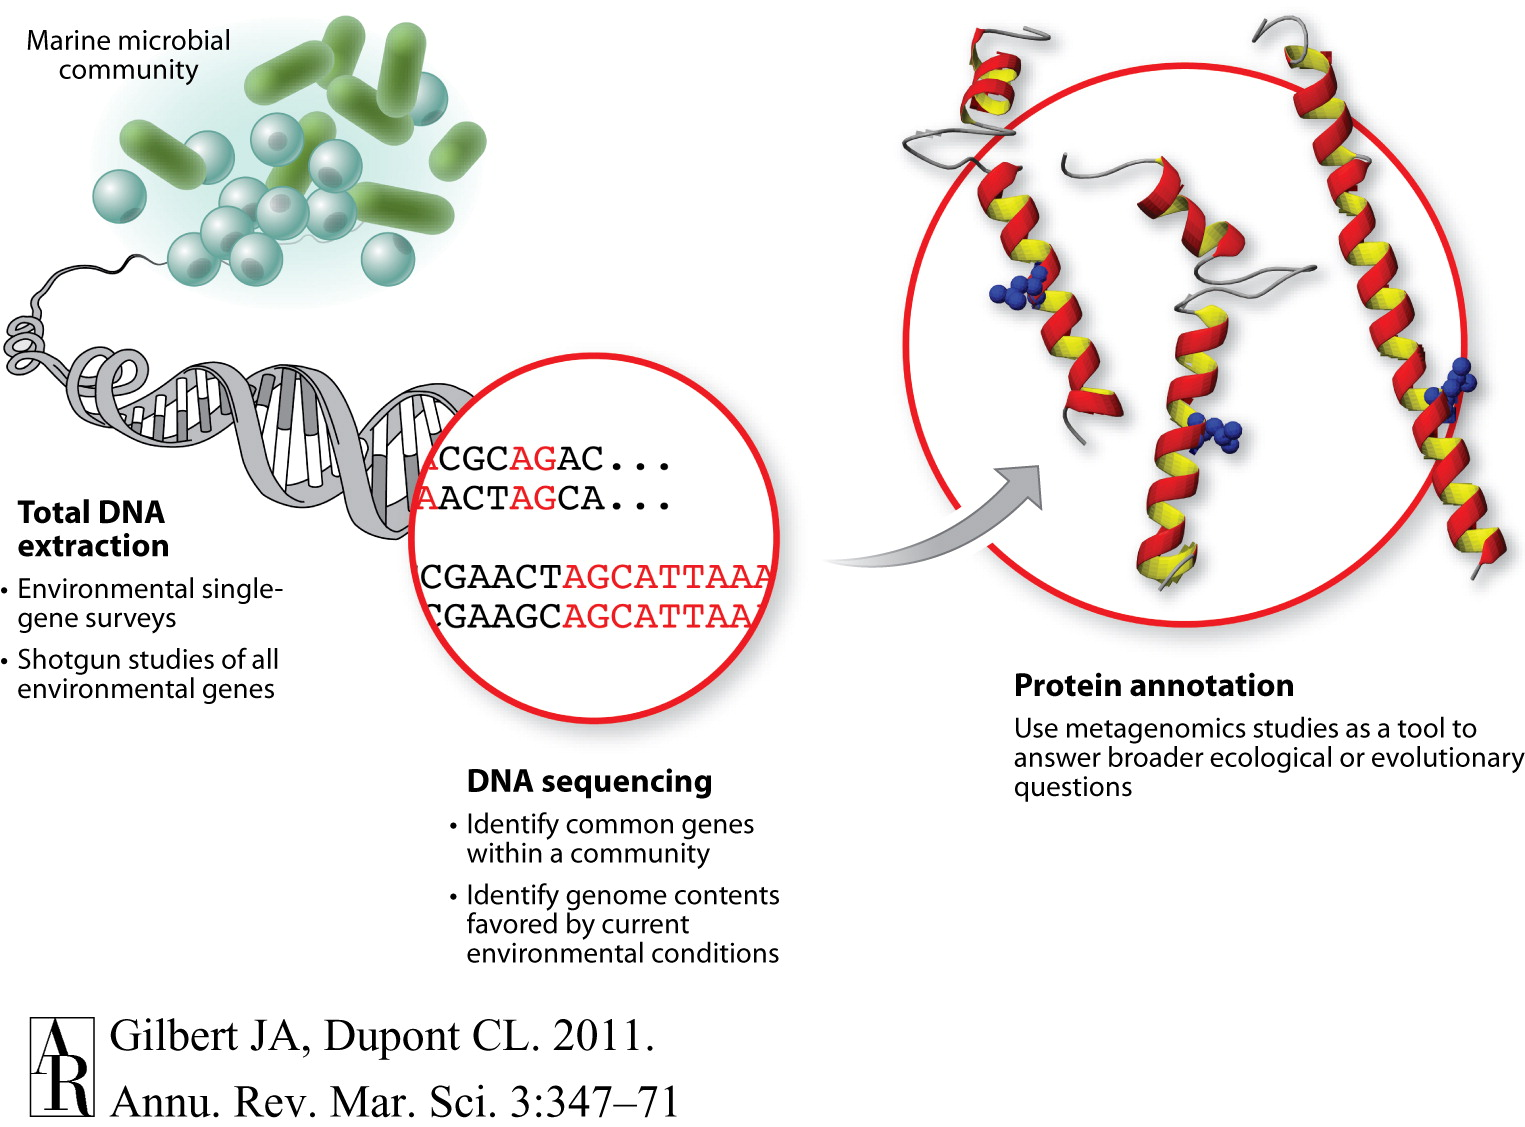
\includegraphics[width=\linewidth,height=15cm,
      keepaspectratio]{Abbildungen/metagenome-steps.jpg}
      \caption{Metagenomik in Schritten}
\end{figure}
   
    
    \subsection{\textrm{Diamond}}    
    Das open source verf\"ugbare Alignierprogramm Diamond \cite{buchfink2014} basiert auf einem Seed- und Extent Algorithmus. Im Seedingschritt werden so gennante Spaced Seeds gesucht, die als Treffer in Anfrage- und Datenbanksequenz gefunden werden sollen (Abb. 2). Das Seeding findet anschlie{\ss}end mit Double Indexing statt. Beim Double Indexing werden sowohl Anfrage- als auch Referenzdatenbanksequenz geindext, was eine geringere Laufzeit durch schnelleres durchsuchen der Datenstrukturen mit sich bringt. Die Indizierung findet bei Diamond $"$on the fly$"$, das hei{\ss}t w\"ahrend des Programmdurchlaufs, statt. Die Treffer, die mit Hilfe der Spaced Seeds gefunden wurden, speichert Diamond in lexikographisch sortierten Listen.
\begin{figure}[h]
\centering
      \noindent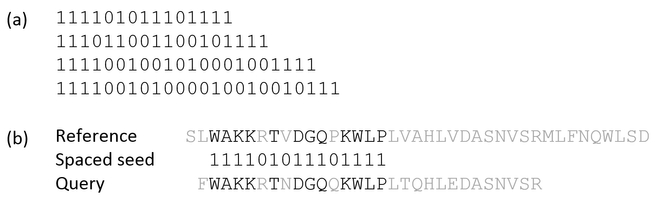
\includegraphics[width=\linewidth,height=15cm,
      keepaspectratio]{Abbildungen/diamond_spacedSeeds.jpg}
      \caption{Spaced Seeds}
\end{figure}
\newline
    Um eine Erweiterung im Extendschritt durchzuf\"uhren, \"uberpr\"uft das Programm, ob der Seed-Treffer gr\"o{\ss}er-gleich 10 Aminos\"auren lang ist. Der Seed wird schlie{\ss}lich mit dem Smith-Waterman Algorithmus erweitert.
\newline
    
    \subsection{\textrm{Lambda}}
    Auch Lambda \cite{hauswedell2014} basiert wie Diamond auf dem Seed- und Extend Algorithmus mit Double Indexing. Im Gegensatz zu Lambda muss die Refernzdatenbank vorgeindext werden und findet nicht w\"ahrend des Programmdurchlaufs statt. Als Datenstrukturen stehen f\"ur die Referenzdatenbank ein Suffixarray und f\"ur die Anfragesequenz ein Radixtree zur Verf\"ugung. Die Speicherung in einem Radixtree erm\"oglicht eine Paralellisierung verschiedener Seeds, was eine zus\"atzliche Zeitersparnis bedeutet. 
    Die Erweiterung erflolgt mit Hilfe des X-drop Algorithmus. 
    \newpage
    \subsection{Ziele}
    
    Das Projekt hat folgende Ziele:
    
    \begin{itemize}
    
      \item Bestimmung und Vergleich der Sensivit"at (Anzahl an korrekt Bestimmten / Anzahl an Sequenzen im Datenset) und Pr\"azision (Anzahl an korrekt Bestimmten / Anzahl an Zugewiesenen) der Programme \textrm{Diamond} 				und \textrm{Lambda}.
      
      \item Bestimmung und Vergleich der ben"otigten Zeit der Programme
      		\textrm{Diamond} und \textrm{Lambda}.

      
    
    \end{itemize}


    \newpage
  \section{Material und Methoden}
    
    \subsection{Material} 
    
      Das durchgef"uhrte Projekt orientiert sich an der Forschungsarbeit von
      Bazinet und Cummings \cite{bazinet2012}. Im 
      Folgenden bezieht sich der Ausdruck "Vorlagepaper"\ auf die Arbeit von
      Bazinet und Cumming. Die Datensets und Datenbanken wurden anhand des 			  Vorlagepapers ausgew"ahlt.
      
      \subsubsection{Datensets}
        Die Experimente wurden mit folgenden Datensets durchgef"uhrt:
        
        \begin{enumerate}
        
          \item \textit{FACS 269bp} $-$ Datenset, original von Strannenheim 			  \textit{et al.} \cite{stranneheim2010}, bestehend aus
          \textbf{27.049 simulierten 454 
          Reads} mit einer durschnittlichen L"ange von \textbf{269 bp}. Die
          im Vorlagepaper angegebene Referenz war nicht mehr aktuell und
          konnte nicht gefunden werden. Das
          Datenset wurde direkt von Herrn Bazinet bereit gestellt. Das 					  bereitgestellte Datenset beinhaltet 72.951 Reads der Spezies 					  \textit{Homo sapiens}. Diese Reads wurden entfernt, so dass das 				  genutzte Datenset 27.049 Reads enth\"alt. Das Datenset setzt sich aus 		  19 bakteriellen und drei viralen Genomen zusammen 							  \cite{bazinet2012}.  
           
          \item \textit{CARMA 265bp} $-$ Datenset bestehend aus
          \textbf{25.000 simulierten 454 Reads} mit einer durschnittlichen 				  L"ange von \textbf{265 bp}, original genutzt von Gerlach und Stoye
          \cite{GerlachStoye2011}.
          Das Datenset
          wurde von der WebCARMA Homepage unter dem Link
          \url{http://wwww.cebitec.uni-bielefeld.de/webcarma.cebitec.uni-
          bielefeld.de/download/simulated_metagenome_454_265bp.fna}\newline
          heruntergeladen. Zusammengesetzt ist das Datenset aus 25 bakteriellen
          Genomen, die sich wie folgt in die einzelnen bakteriellen Phyla 				  verteilen: 73,0\% Proteobacteria; 12,9\% Firmicutes; 7,8\% 					  Cyanobacteria; 5,2\% Actinobacteria; 1,0\% Clamydiae 							  \cite{bazinet2012}.
          
          \item \textit{Metaphyler 300bp} $-$ Datenset bestehend aus 
          \textbf{73.086 simulierten
          Reads} von 31 phylogenetischen Markern bakterieller Genome mit 			  	  einer durschnittlichen L"ange von \textbf{300 bp}. Urspr\"unglich 			  genutzt von Liu \textit{et al.} \cite{Liu2010}. Das
          Datenset konnte anhand der im Vorlagepaper angegebenen Referenz nicht 
          korrekt ermittelt werden. Die Rechercheergebnisse
          ergaben ein Datenset bestehend aus 40.039 Reads mit einer 
          durchschnittlichen L"ange von 645 bp. Das korrekte
          Datenset wurde direkt von Herrn Bazinet bereit gestellt. 
          Die Verteilung in die bakteriellen Phyla setzt sich folgenderma"sen 			  zusammen: 47.0\% Proteobacteria; 21.9\% Firmicutes; 9.7\% 					  Actinobacteria; 4.8\% Bacteroidetes; 3.9\% Cyanobacteria; 2.2\% 				  Tenericutes; 1.9\% Spirochaetes; 1.3\% Chlamydiae; 0.9\% 						  Thermotogae; 0.9\% Chlorobi \cite{bazinet2012}. 
          
          \item \textit{PhymmBL 243bp} $-$ Datenset bestehend aus 
          \textbf{80.215 RefSeq
          Reads} mit einer durschnittlichen L"ange von
          \textbf{243 bp}. Das Datenset, original genutzt von Brady und 
          Salzberg \cite{bradysalzberg2009},  
          konnte anhand der im Vorlagepaper angegebenen Referenz nicht 
          korrekt ermittelt werden. Die Rechercheergebnisse
          ergaben ein Datenset bestehend aus 73.252 Reads mit einer 
          durchschnittlichen L"ange von 204 bp. Das korrekte
          Datenset wurde direkt von Herrn
          Bazinet bereit gestellt.  
          
          \item \textit{PhyloPythia 969bp} $-$ simMC Datenset bestehend aus
          \textbf{114.457 Reads} mit einer durschnittlichen L"ange von
          \textbf{969 bp}, original von Patil \textit{et al.} \cite{patil2011}. 		  Das im Vorlagepaper verwendete Datenset 
          "PhyloPythia"\ bestehend aus 124.941 Reads mit einer 
          durchschnittlichen L"ange von 961 bp konnte
          auch mit Hilfe von Herrn Bazinet nicht ermittelt werden.
          Das Datenset wurde von der JGI Homepage unter dem Link
          \url{http://fames.jgi-psf.org/Retrieve_data.html} heruntergeladen.  
          
          \item \textit{RAIphy 233bp} $-$ Datenset bestehend aus
          \textbf{477.000 RefSeq Reads} mit einer durschnittlichen L"ange von
          \textbf{233 bp}, original von Nalbantoglu \textit{et al.} 					  \cite{nalbantoglu2011}. Das im Vorlagepaper verwendete Datenset 
          "RAIphy"\ bestehend aus 477.000 Reads mit einer 
          durchschnittlichen L"ange von 238 bp konnte
          mit der angegebenen Referenz nicht ermittelt werden.
          Das im Projekt verwendete Datenset wurde von Herrn Bazinet zur
          Verf"ugung gestellt.
          
        \end{enumerate}
        
      \subsubsection{Datenbank}
      F\"ur die Suche wurde die Datenbank UniProtKB/Swiss-Prot von UniProt 			  verwendet \cite{bairoch2004}.
      Diese wurde unter dem Link \url{http://www.uniprot.org/downloads}
      heruntergeladen.
      Die Datenbank besteht aus 549.646 Sequenzen mit einer durchschnittlichen 
      L\"ange von 356.56bp.
      \subsubsection{Programme}
        Im Projekt wurden folgende Programme verwendet:
        
        \begin{enumerate}
          
          \item \textbf{Lambda} $-$ Das Programm Lambda (Version 0.9.2) wurde 			  von der GitHub Seite mit dem Link 											  \url{https://github.com/seqan/lambda.git} heruntergeladen 					  \cite{hauswedell2014}. Dabei wurde wie folgt vorgegangen:
          \begin{itemize}
            \item[\$] git clone \url{https://github.com/seqan/lambda.git}
            \item[\$] cd lambda
            \item[\$] mkdir build
            \item[\$] cmake 																    -DCMAKE\_C\_COMPILER=/usr/local/zbhtools/gcc/gcc-5.1.0/bin/gcc 
            -DCMAKE\_CXX\_COMPILER=/usr/local/zbhtools/gcc/gcc-5.1.0/bin/g++ 
            -DCMAKE\_INSTALL\_PREFIX=\$/work/gi/software 
            \item[\$] make -j2													   
          \end{itemize}
          Um das Programm Lambda ausf\"uhren zu k\"onnen musste die 					  UniProtKB/Swiss-Prot Datenbank zun\"achst indiziert werden. Dazu 				  wurde das Programm "lambda\_indexer"\ verwendet, welches in dem oben 		  genannten Packet enthalten ist. Folgender Aufruf wurde verwendet:
          \begin{itemize}
            \item[\$] lambda\_indexer -d uniprot\_sprot.fasta
          \end{itemize}
          Die jeweiligen Datensets (s.o.) wurden gegen die indizierte 					  Datenbank mit dem Befehl
          \begin{itemize}
            \item[\$] lambda -q QUERY.fasta -d DATABASE.fasta [-o output.m8]
          \end{itemize}
          aligniert.
          
          
          \item \textbf{Diamond} $-$ Das Programm Diamond (Version 0.7.9) 				  wurde 
          von der GitHub Seite mit dem Link
          \url{https://github.com/bbuchfink/diamond.git} heruntergeladen
          \cite{buchfink2014}. Es wurde folgenderma\ss{en} verfahren:
          \begin{itemize}
            \item[\$] git clone \url{https://github.com/bbuchfink/diamond.git}
            \item[\$] cd diamond
            \item[\$] mkdir build
            \item[\$] cmake 																-DCMAKE\_INSTALL\_PREFIX=\$/work/gi/software/diamond
            \item[\$] make install
		  \end{itemize}
		  Mit dem Aufruf
		  \begin{itemize}
		    \item[\$] diamond makedb --in uniprot\_sprot.fasta -d 							diamonduniprot\_sprot.fasta.dmnd
		  \end{itemize}
		  wurde die bin\"are Diamond-Datenbank aus der UniProtKB/Swiss-Prot
		  Datenbank erstellt.\newline
		  Die jeweiligen Datensets (s.o.) wurden gegen die zuvor erstellte 				  Diamond-Datenbank mit dem Befehl
		  \begin{itemize}
		    \item[\$] diamond blastx -d DIAMOND\_DATABASE.dmnd -q QUERY.fasta 				-a OUTPUT -t <temporary directory> 
		  \end{itemize}
		  aligniert.		             
          
          \item \textbf{MEGAN5} $-$ Das Programm MEGAN5 (Version 5.10.7) wurde 
          von der Website \url{http://ab.inf.uni-										  tuebingen.de/data/software/megan5/download/welcome.html}
          heruntergeladen \cite{huson2011}. Die ben\"otigte akademische
          Lizenz wurde uns von Herrn Dr. Giorgio Gonella zur Verf\"ugung 
          gestellt. MEGAN5 ist ein Programm mit einer graphischen 						  Benutzeroberfl\"ache. Das Programm ben\"otigt eine "map"\ gegen die
          es die Eingabereads vergleicht. Es konnte nicht die 				  			  voreingestellte "map"\ genutzt werden, da diese gegen GI-Nummern 				  sucht, die Ausgabe von Lambda und Diamond jedoch durch die Nutzung 			  der UniProtKB/Swiss-Prot Datenbank keine GI-Nummern sondern sp-				  Nummern generiert. Aus diesem Grund wurde die $"$idmapping.dat"\ von 		  der Website 									\url{ftp://ftp.uniprot.org/pub/databases/uniprot/current_release/knowledgebase/idmapping/} 		  heruntergeladen. Diese wurde anschlie{\ss}end gek\"urzt, so dass nur 		  die Taxa enthalten waren, die auch in der UniProtKB/Swiss-Prot 				  Datenbank vorkommen. 
          
        \end{enumerate}
    \subsection{Methoden}
      \subsubsection{Vorarbeit}
      \subsubsection{Programmausgabe}
      \subsubsection{Megan}
      \subsubsection{Newick}
      \subsubsection{Genauigkeitsberechnungen}
    
  
    \newpage
  \section{Ergebnisse}
  \subsection{Distanzverteilung}
  
  Abbildungen 3 - 8 zeigen die Distanzverteilungen der Reads, welche mithilfe des newick-parser ermittelt wurden. Um einen direkten Vergleich von Diamond und Lambda vornehmen zu k\"onnen, wurden pro Datensatz die Ergebnisse beider Programme gegeneinander gestellt. Die Verteilung der Datens\"atze Carma (Abb. 3), FACS (Abb. 4) und PhyloPythia (Abb. 5) zeigt die gemeinsame Tendenz, dass die Ausgabe des Programms Diamond eine hohe Anzahl Reads mit einer geringen Distanz aufweist. Die Ausgaben von Lambda zeigen erst bei einer Distanzgr\"o{\ss}e von gr\"o{\ss}er als 4 bemerkenswerte Readanzahlen.
  
    \begin{figure}[H]
      \centering
      \noindent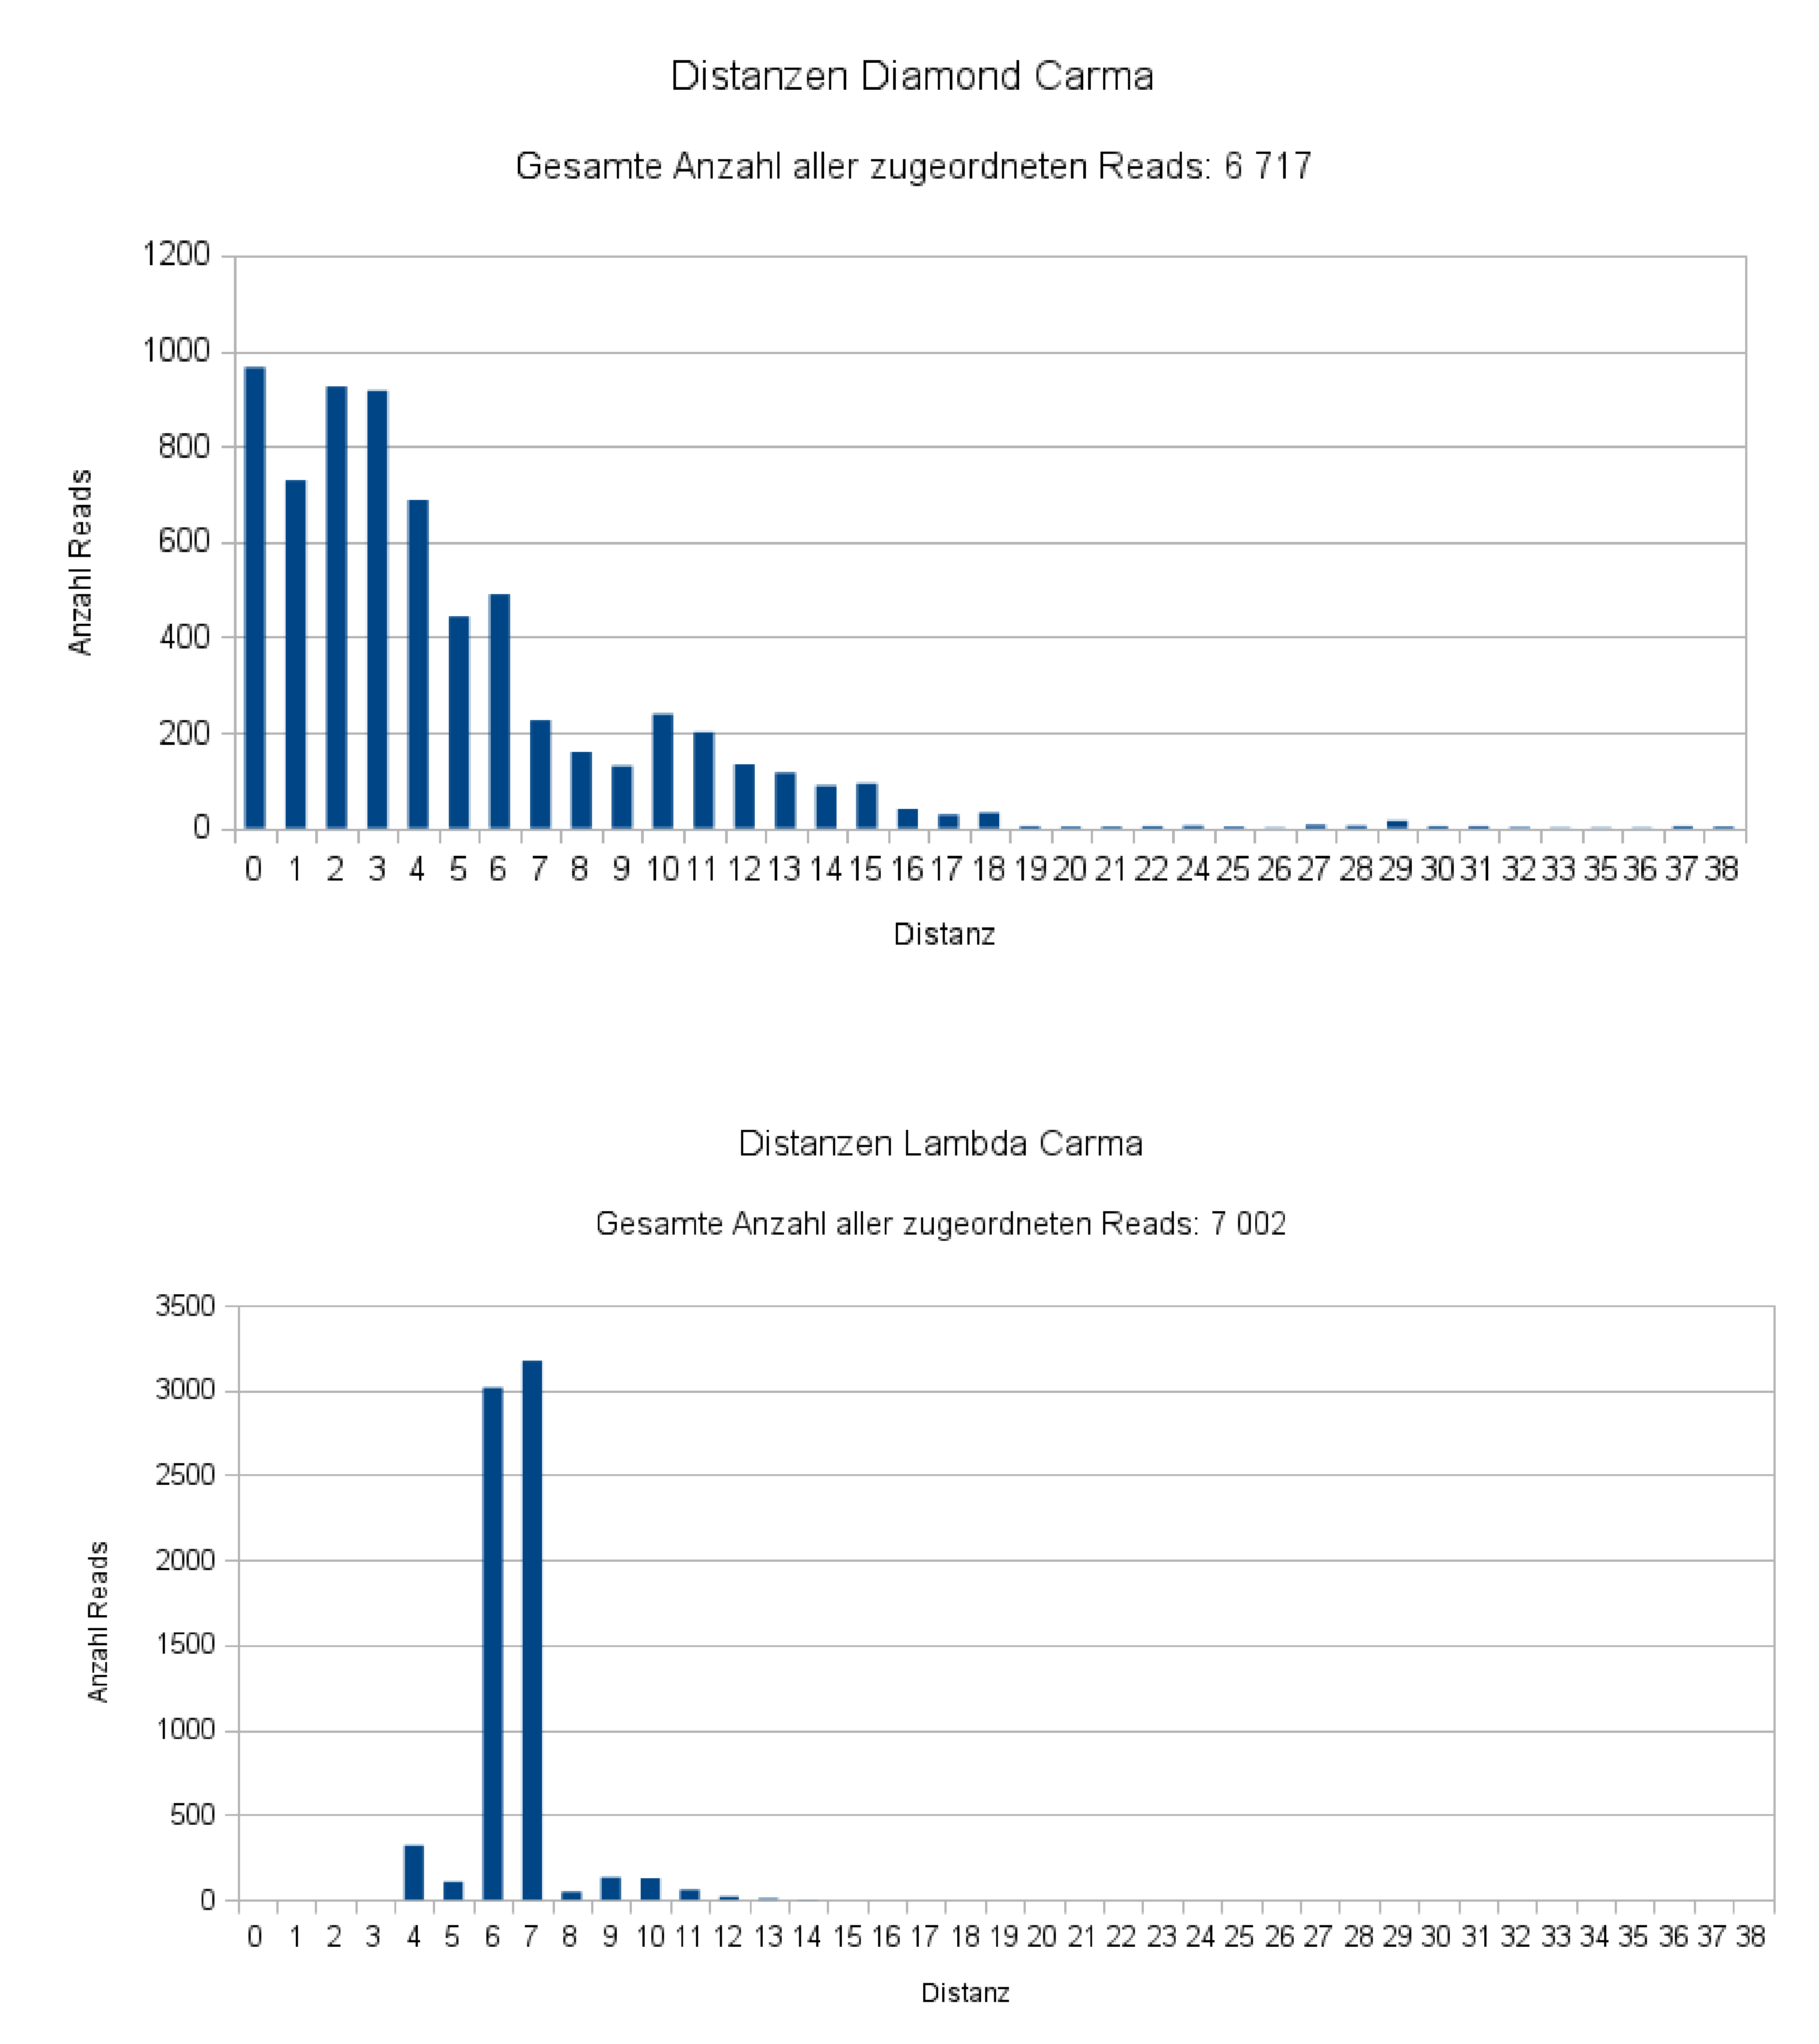
\includegraphics[width=\linewidth,height=13cm,
      keepaspectratio]{Abbildungen/Carma_Distanzen_both.png}
      \caption[Distanzverteilung der Reads: Carma Datensatz.]{\small{Distanzverteilung der Reads: Carma Datensatz.\newline \textbf{Oben}: Ausgabe Diamond. \textbf{Unten}: Ausgabe Lambda.}}
      \centering     
    \end{figure}

    \begin{figure}[H]
      \centering
      \noindent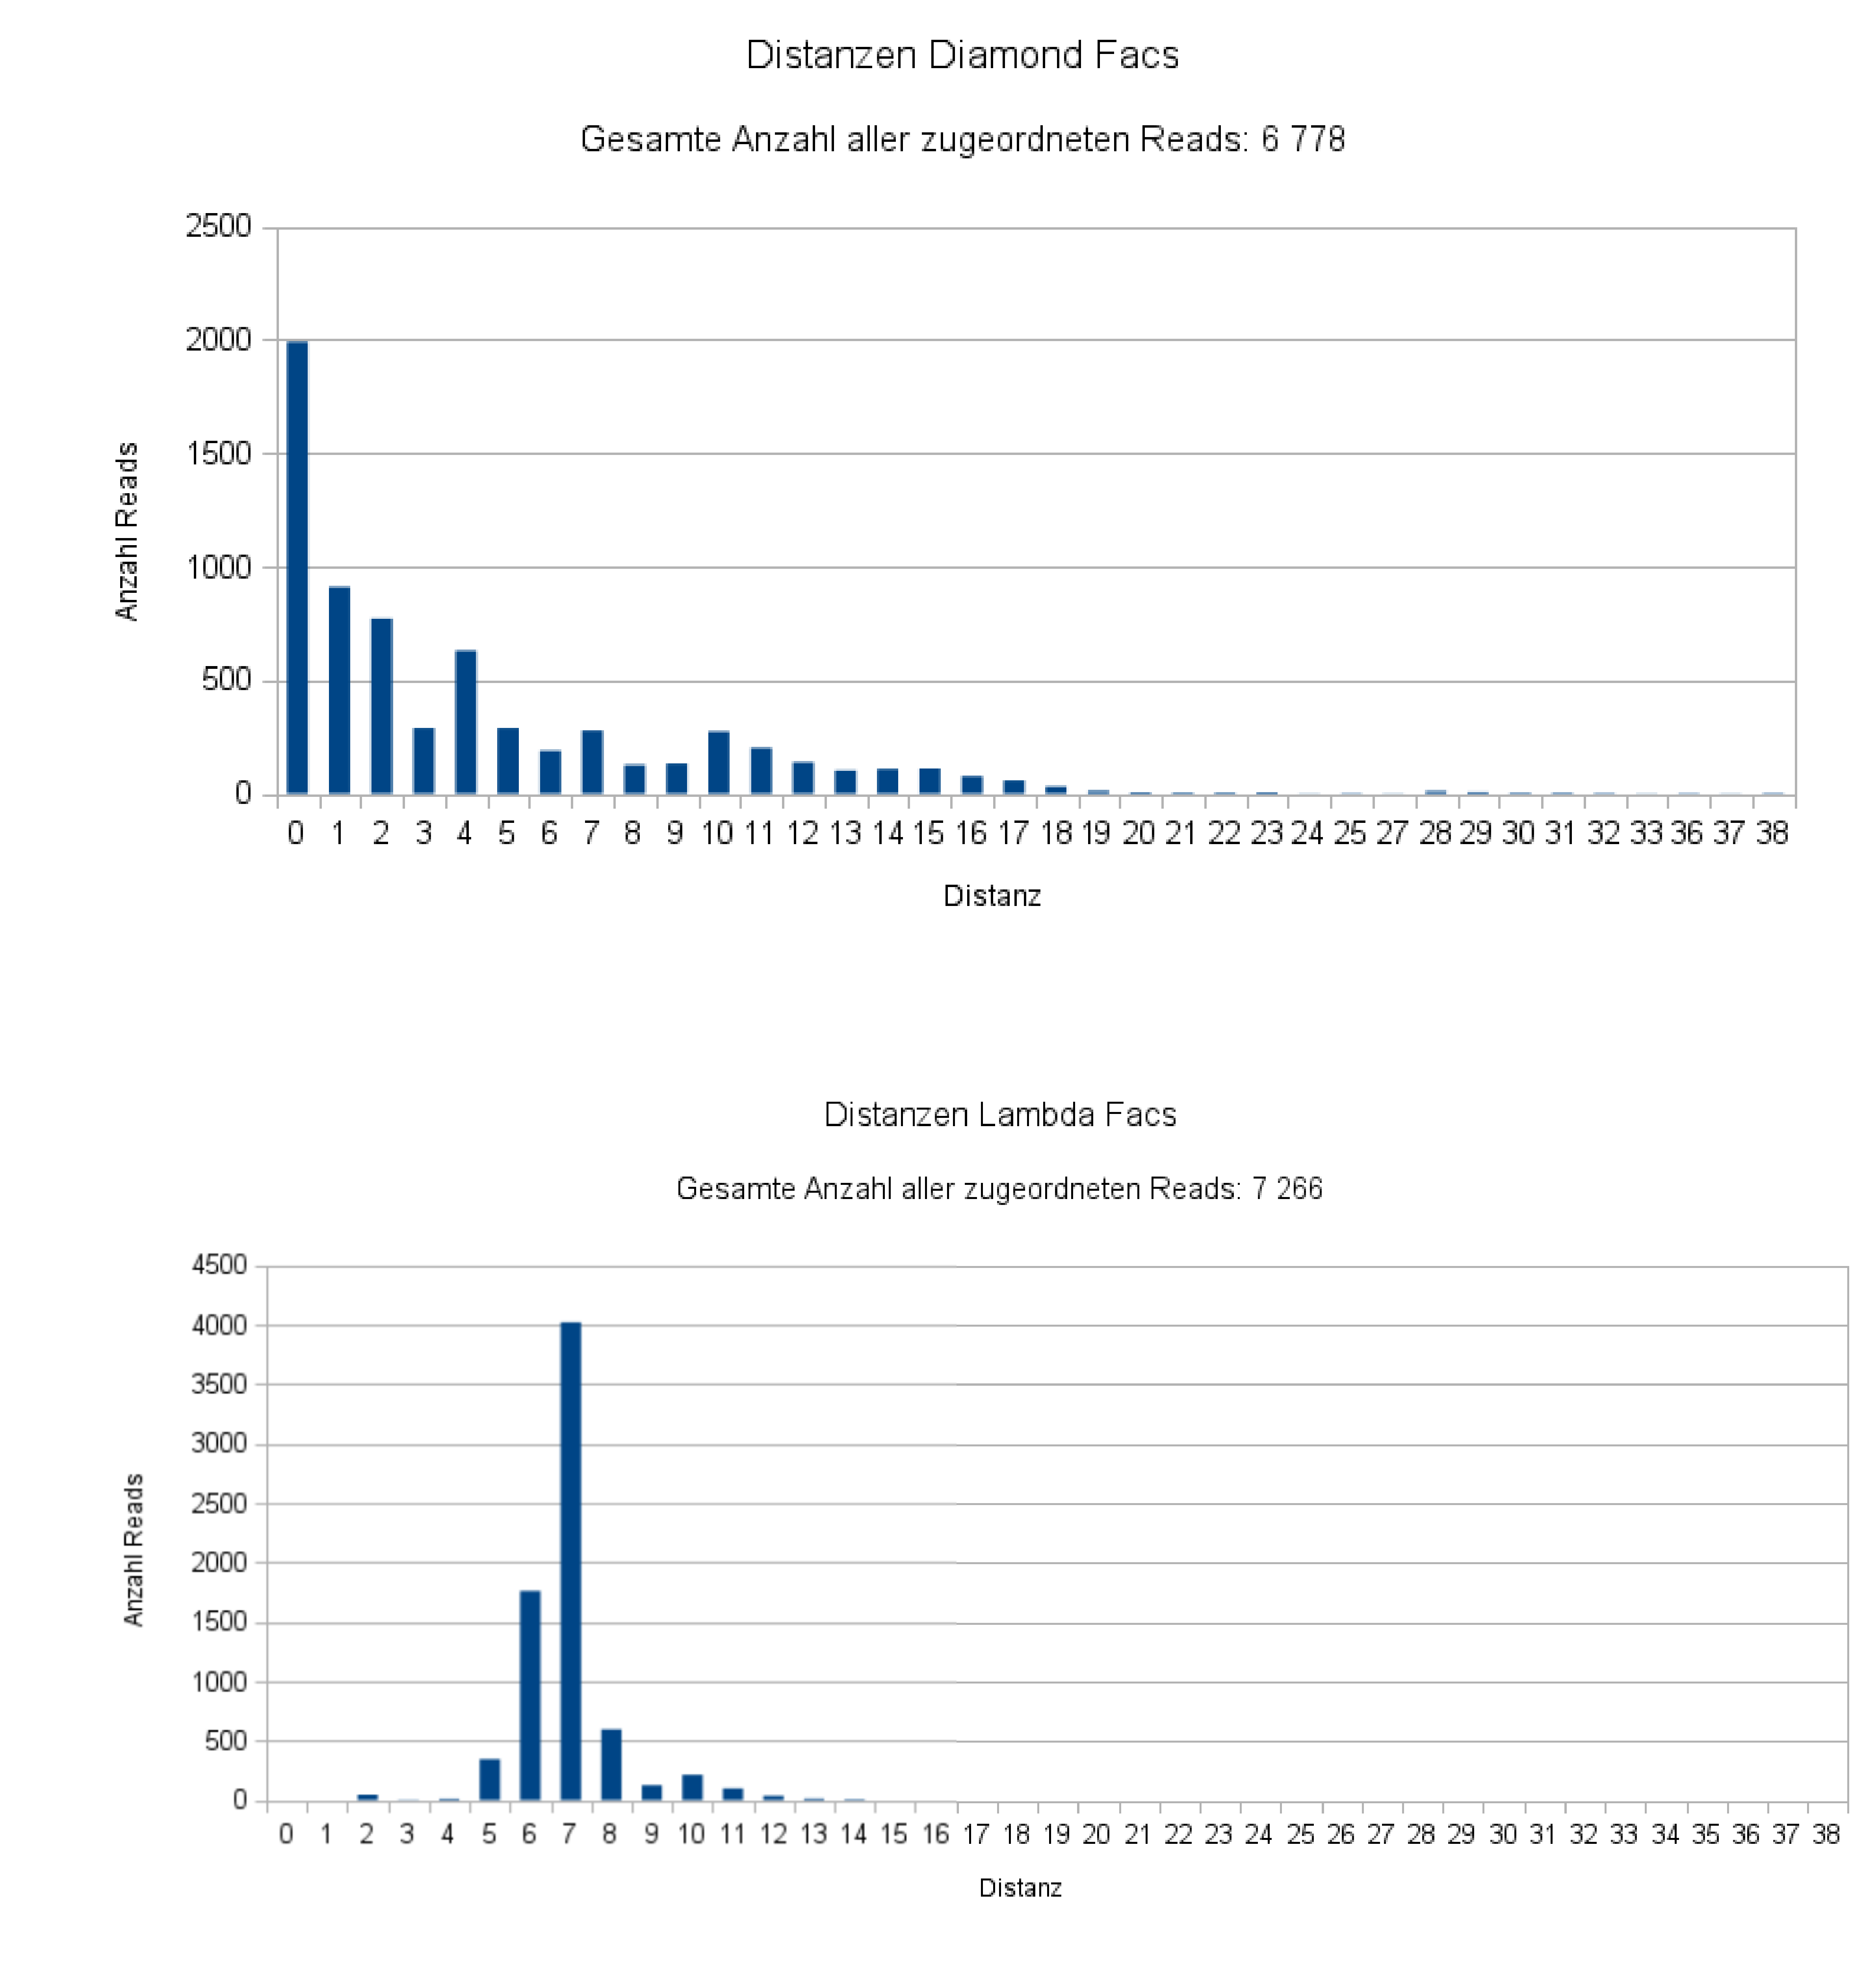
\includegraphics[width=\linewidth,height=13cm,
      keepaspectratio]{Abbildungen/Facs_Distanzen_both.png}
      \caption[Distanzverteilung der Reads: FACS Datensatz.]{\small{Distanzverteilung der Reads: FACS Datensatz.\newline \textbf{Oben}: Ausgabe Diamond. \textbf{Unten}: Ausgabe Lambda.}}
    \end{figure}
    
     \begin{figure}[H]
      \centering
      \noindent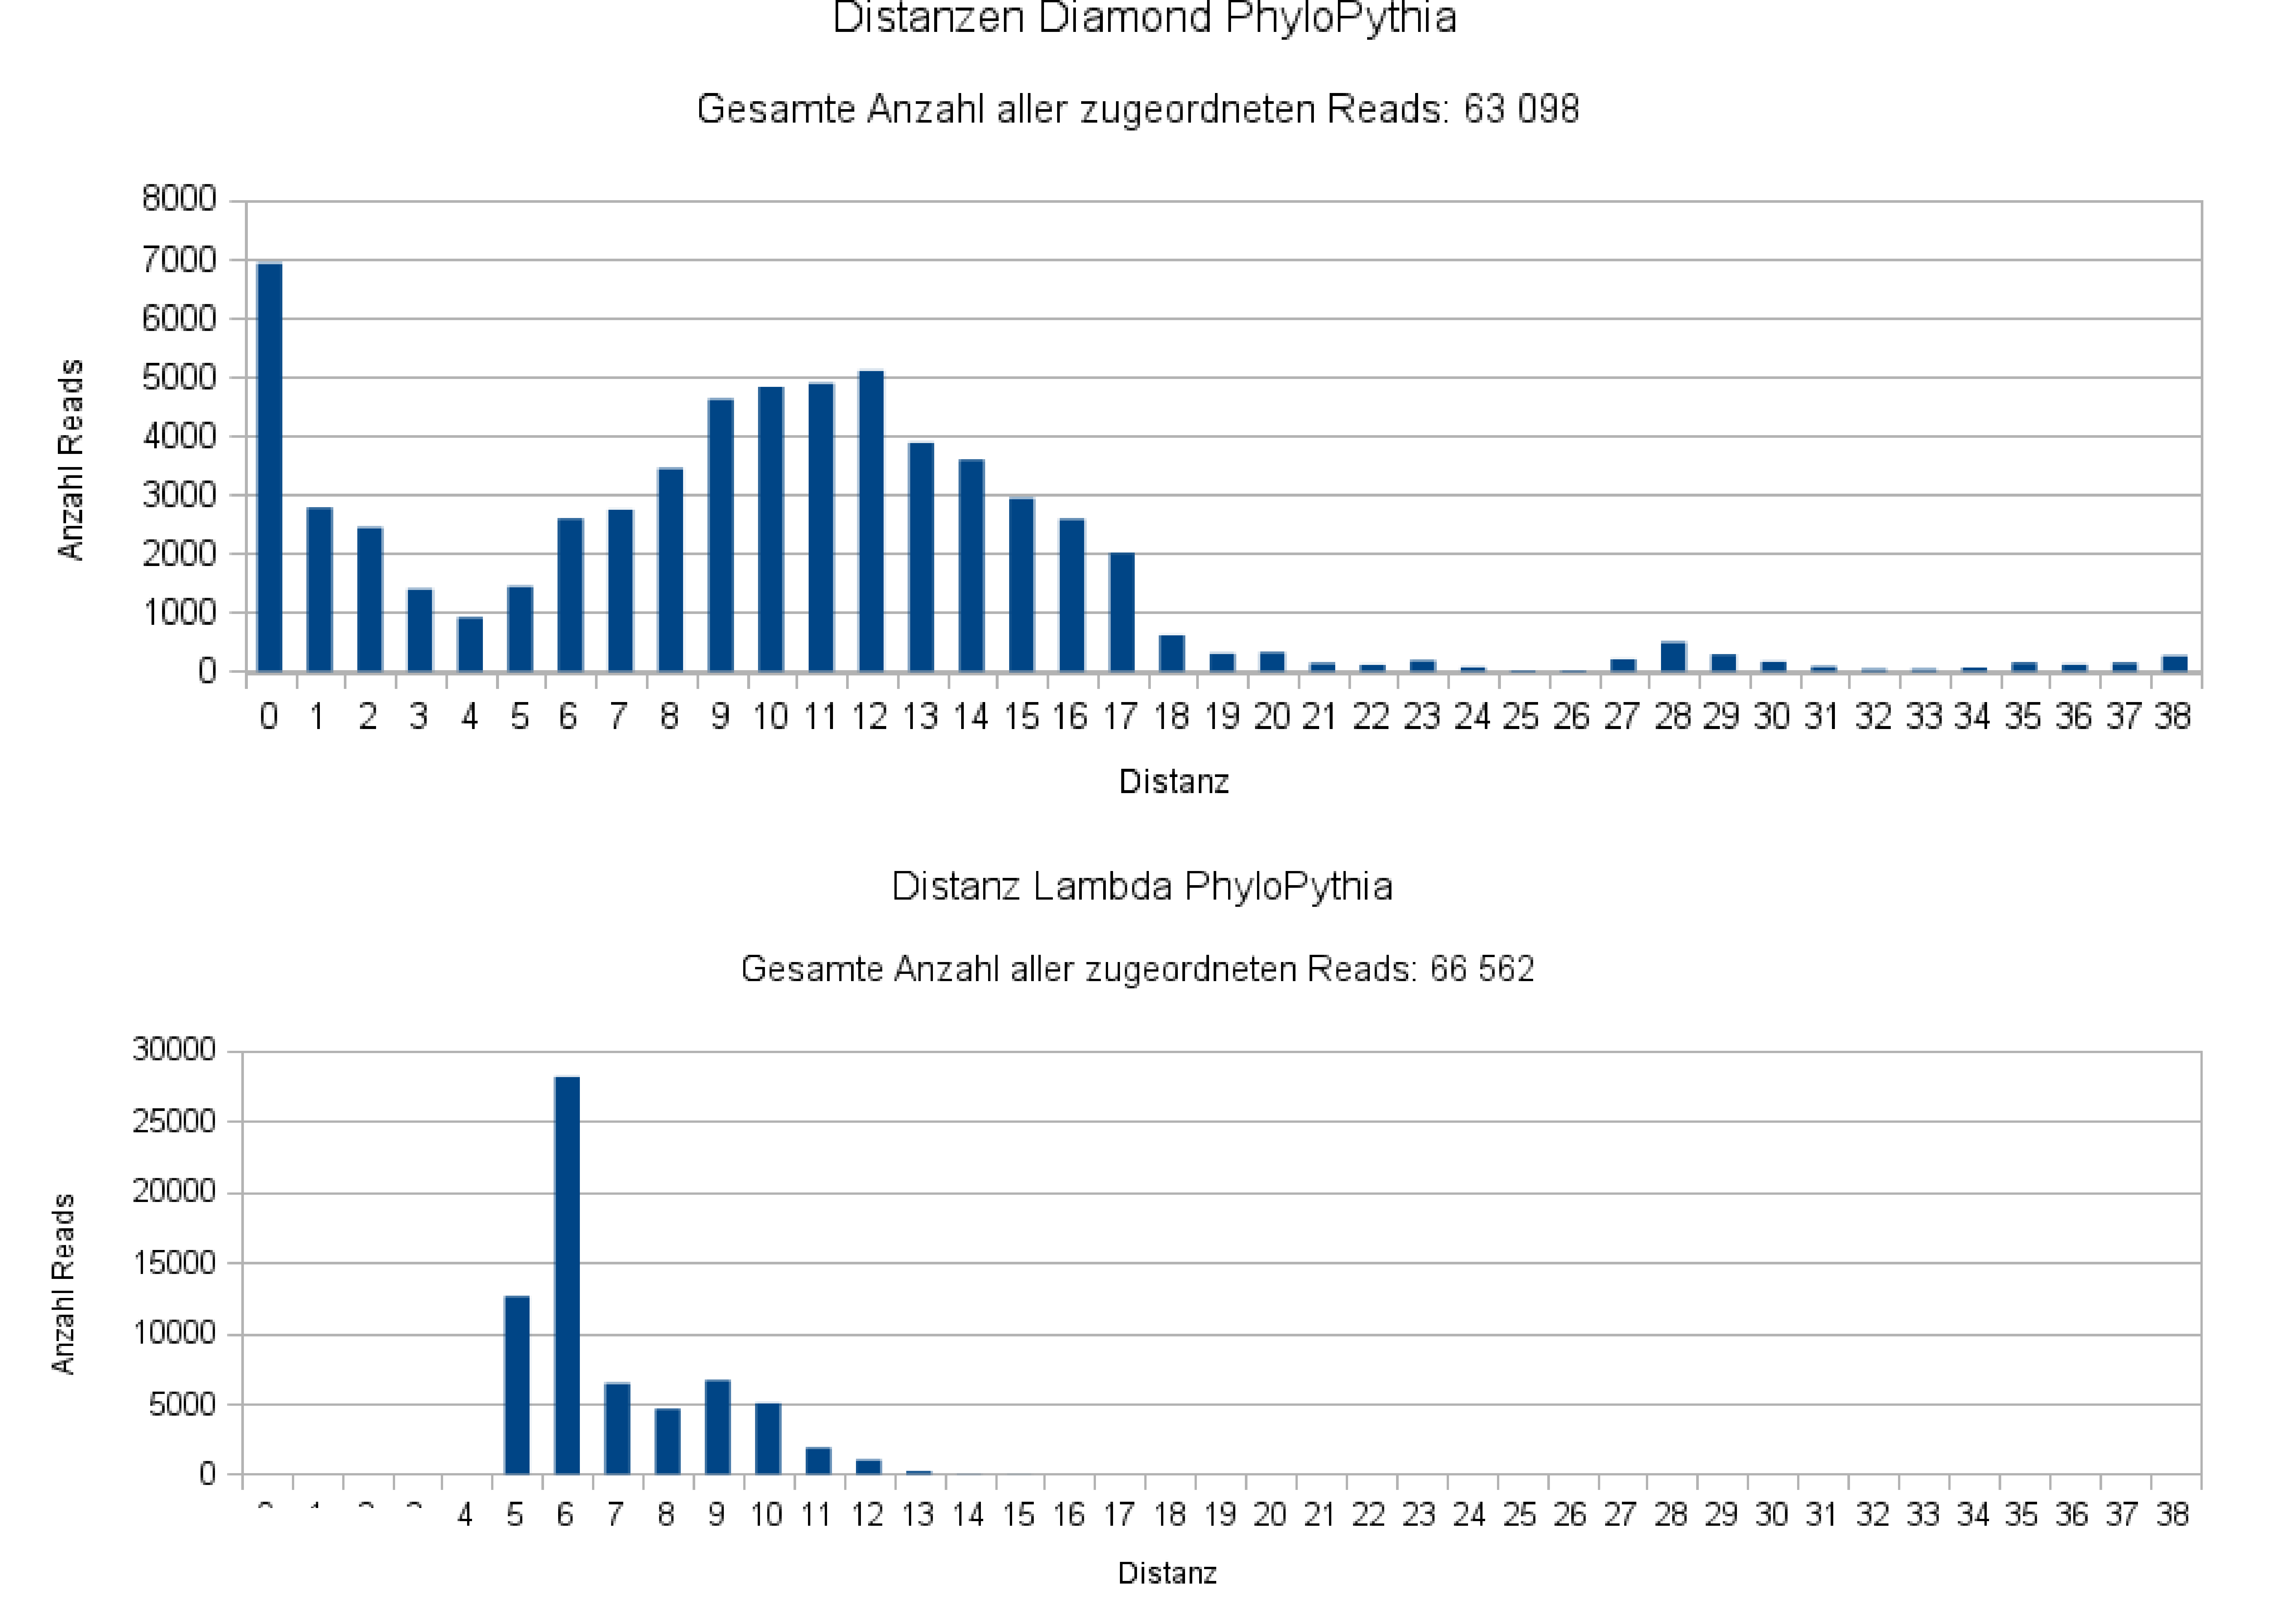
\includegraphics[width=\linewidth,height=20cm,
      keepaspectratio]{Abbildungen/PhyloPythia_Distanzen_both.png}
      \caption[Distanzverteilung der Reads: PhyloPythia Datensatz.]{\small{Distanzverteilung der Reads: PhyloPythia Datensatz.\newline \textbf{Oben}: Ausgabe Diamond. \textbf{Unten}: Ausgabe Lambda.}}
    \end{figure}
    Die jeweiligen Ergebnisse der beiden Programme f\"ur die \"ubrigen drei 		Datens\"atze (Abb. 6-8) \"ahneln sich sehr. Auff\"allig ist hier, dass
    die Zuweisung der Reads bei beiden Programmen f\"ur die Datens\"atze 			Metaphyler (Abb. 6) und PhymmBL (Abb. 7) erst nennenswerte Readanzahlen 		bei einer Distanz von gr\"o{\ss}er als 4 erzeugen. F\"ur den Datensatz
    RAIphy k\"onnen bei beiden Programmen hohe Readanzahlen bei einer Distanz
    von 0 beobachtet werden.    

     \begin{figure}[H]
      \centering
      \noindent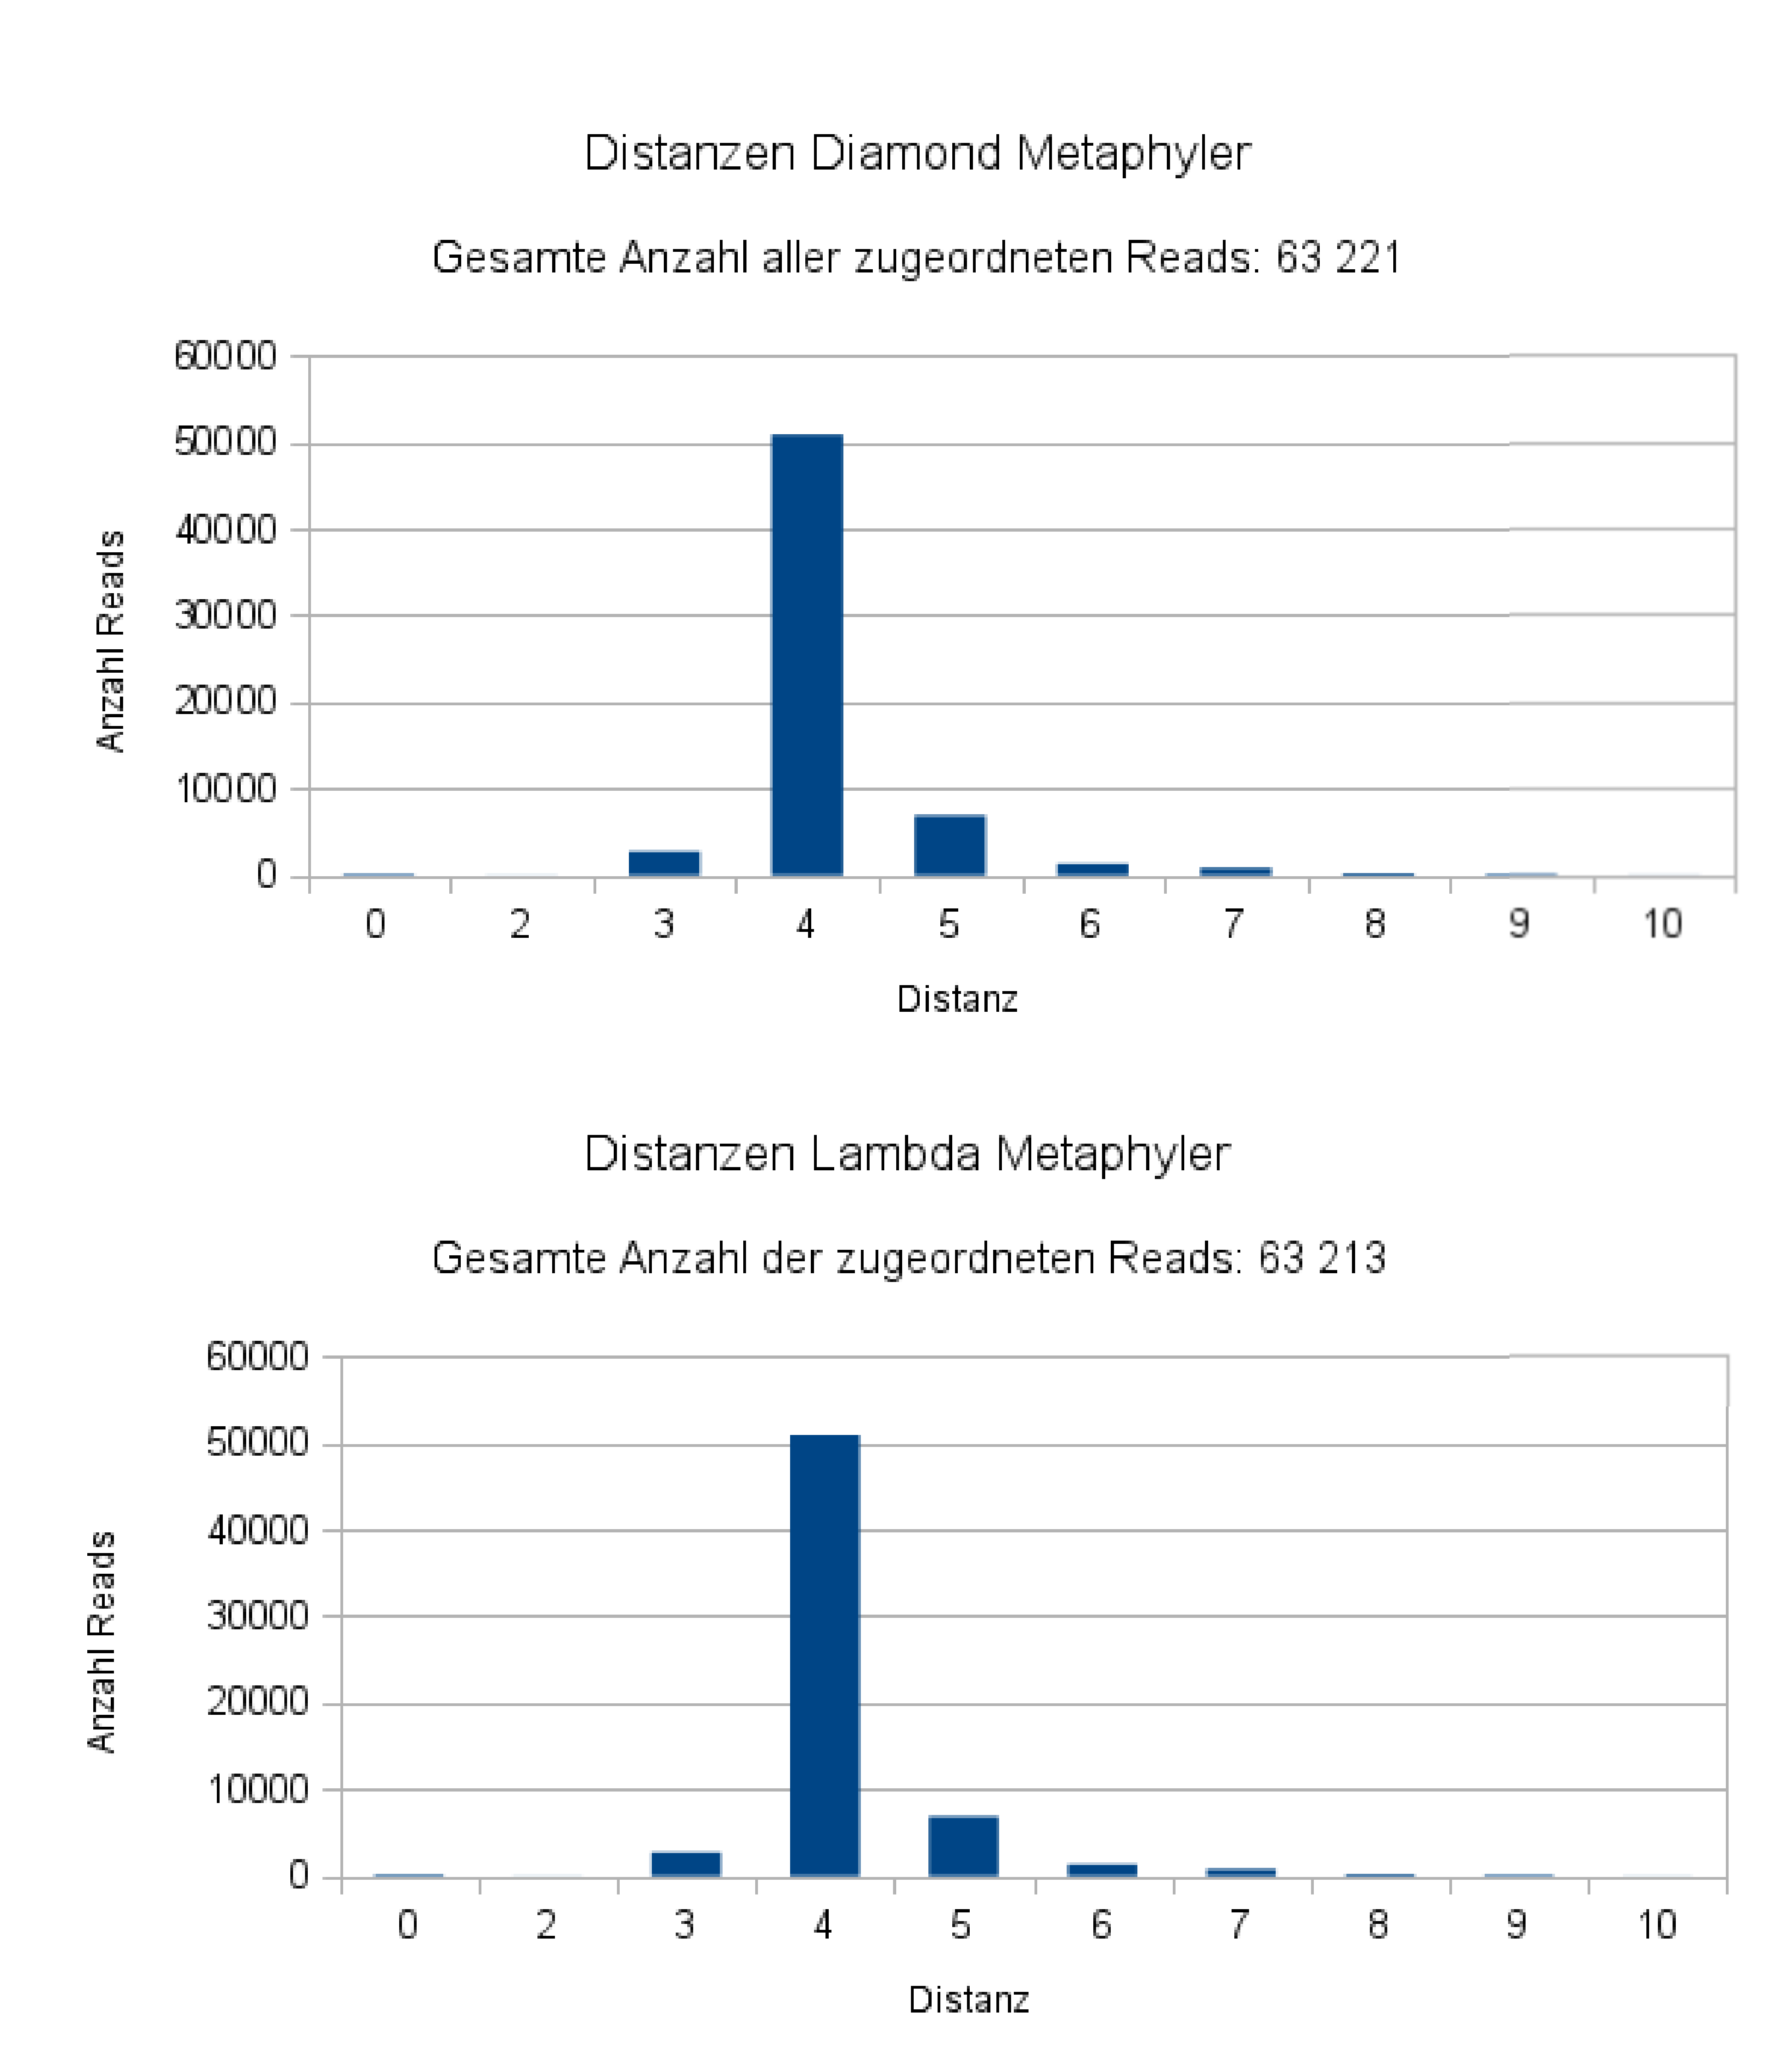
\includegraphics[width=\linewidth,height=15cm,
      keepaspectratio]{Abbildungen/Metaphyler_Distanzen_both.png}
      \caption[Distanzverteilung der Reads: Metaphyler Datensatz.]{\small{Distanzverteilung der Reads: Metaphyler Datensatz.\newline \textbf{Oben}: Ausgabe Diamond. \textbf{Unten}: Ausgabe Lambda.}}
    \end{figure}


     \begin{figure}[H]
      \centering
      \noindent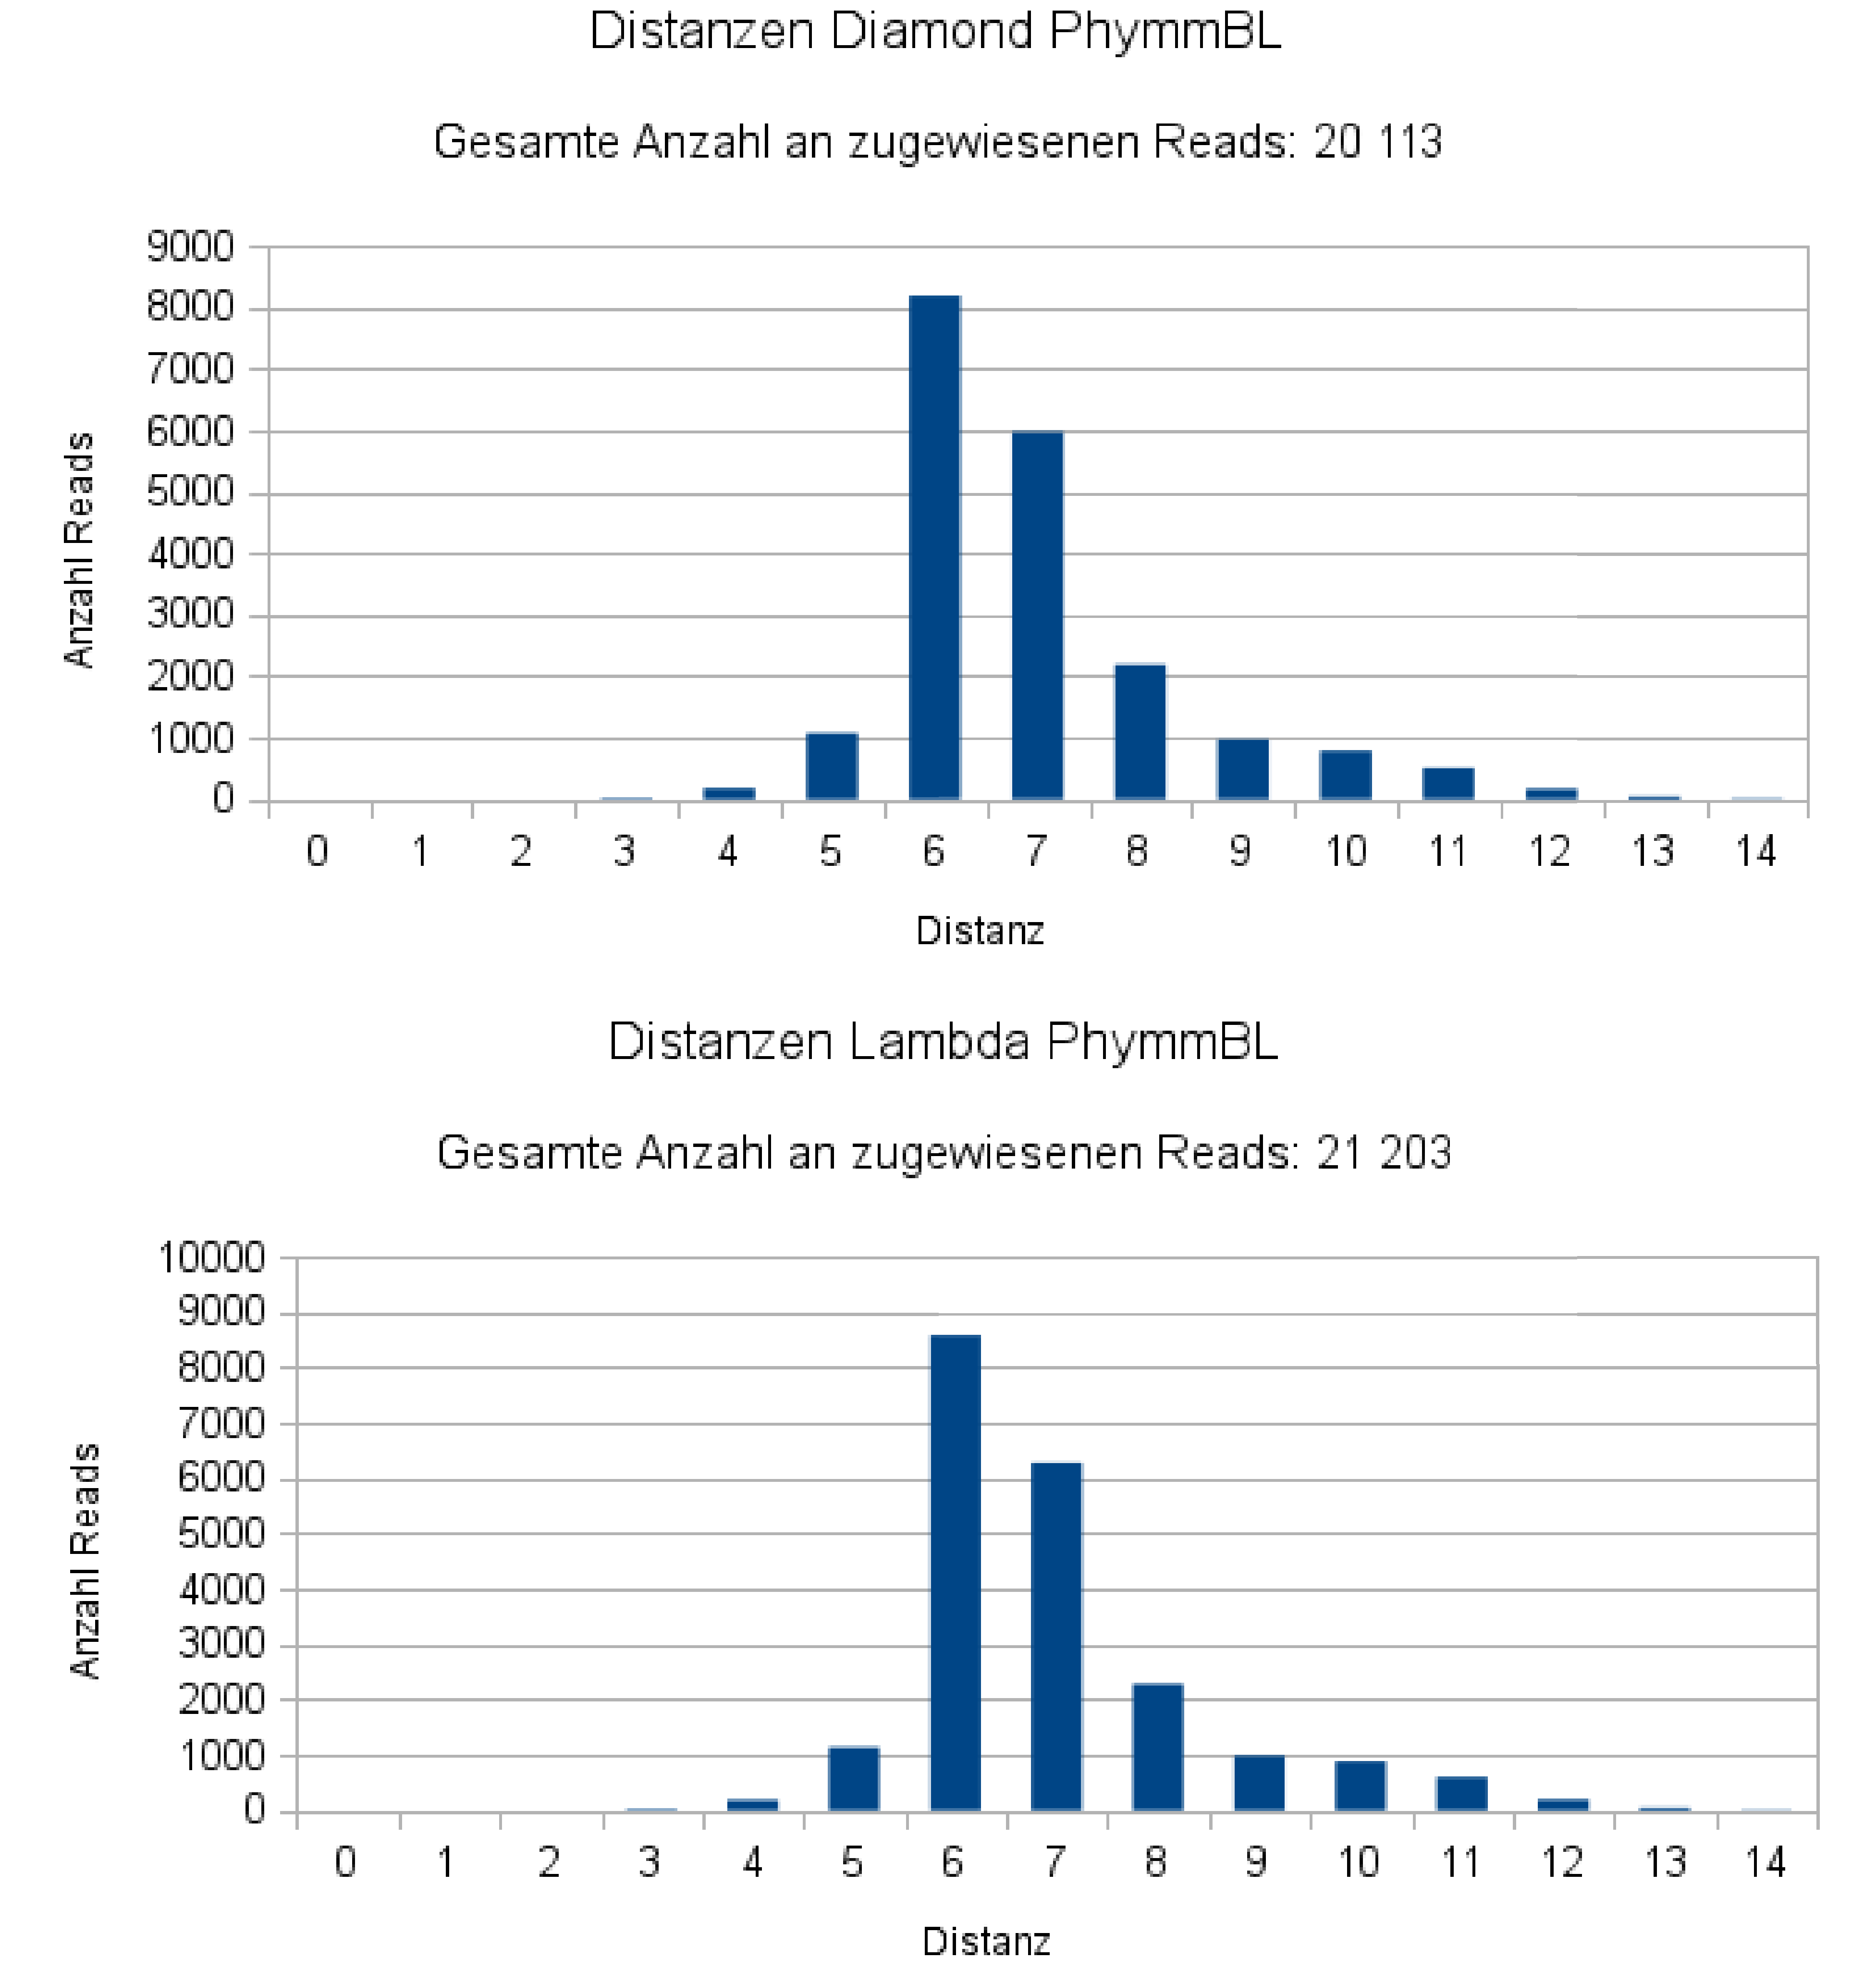
\includegraphics[width=\linewidth,height=15cm,
      keepaspectratio]{Abbildungen/PhymmBL_Distanzen_both.png}
      \caption[Distanzverteilung der Reads: PhymmBL Datensatz.]{\small{Distanzverteilung der Reads: PhymmBL Datensatz.\newline \textbf{Oben}: Ausgabe Diamond. \textbf{Unten}: Ausgabe Lambda.}}
    \end{figure}
    
     \begin{figure}[H]
      \centering
      \noindent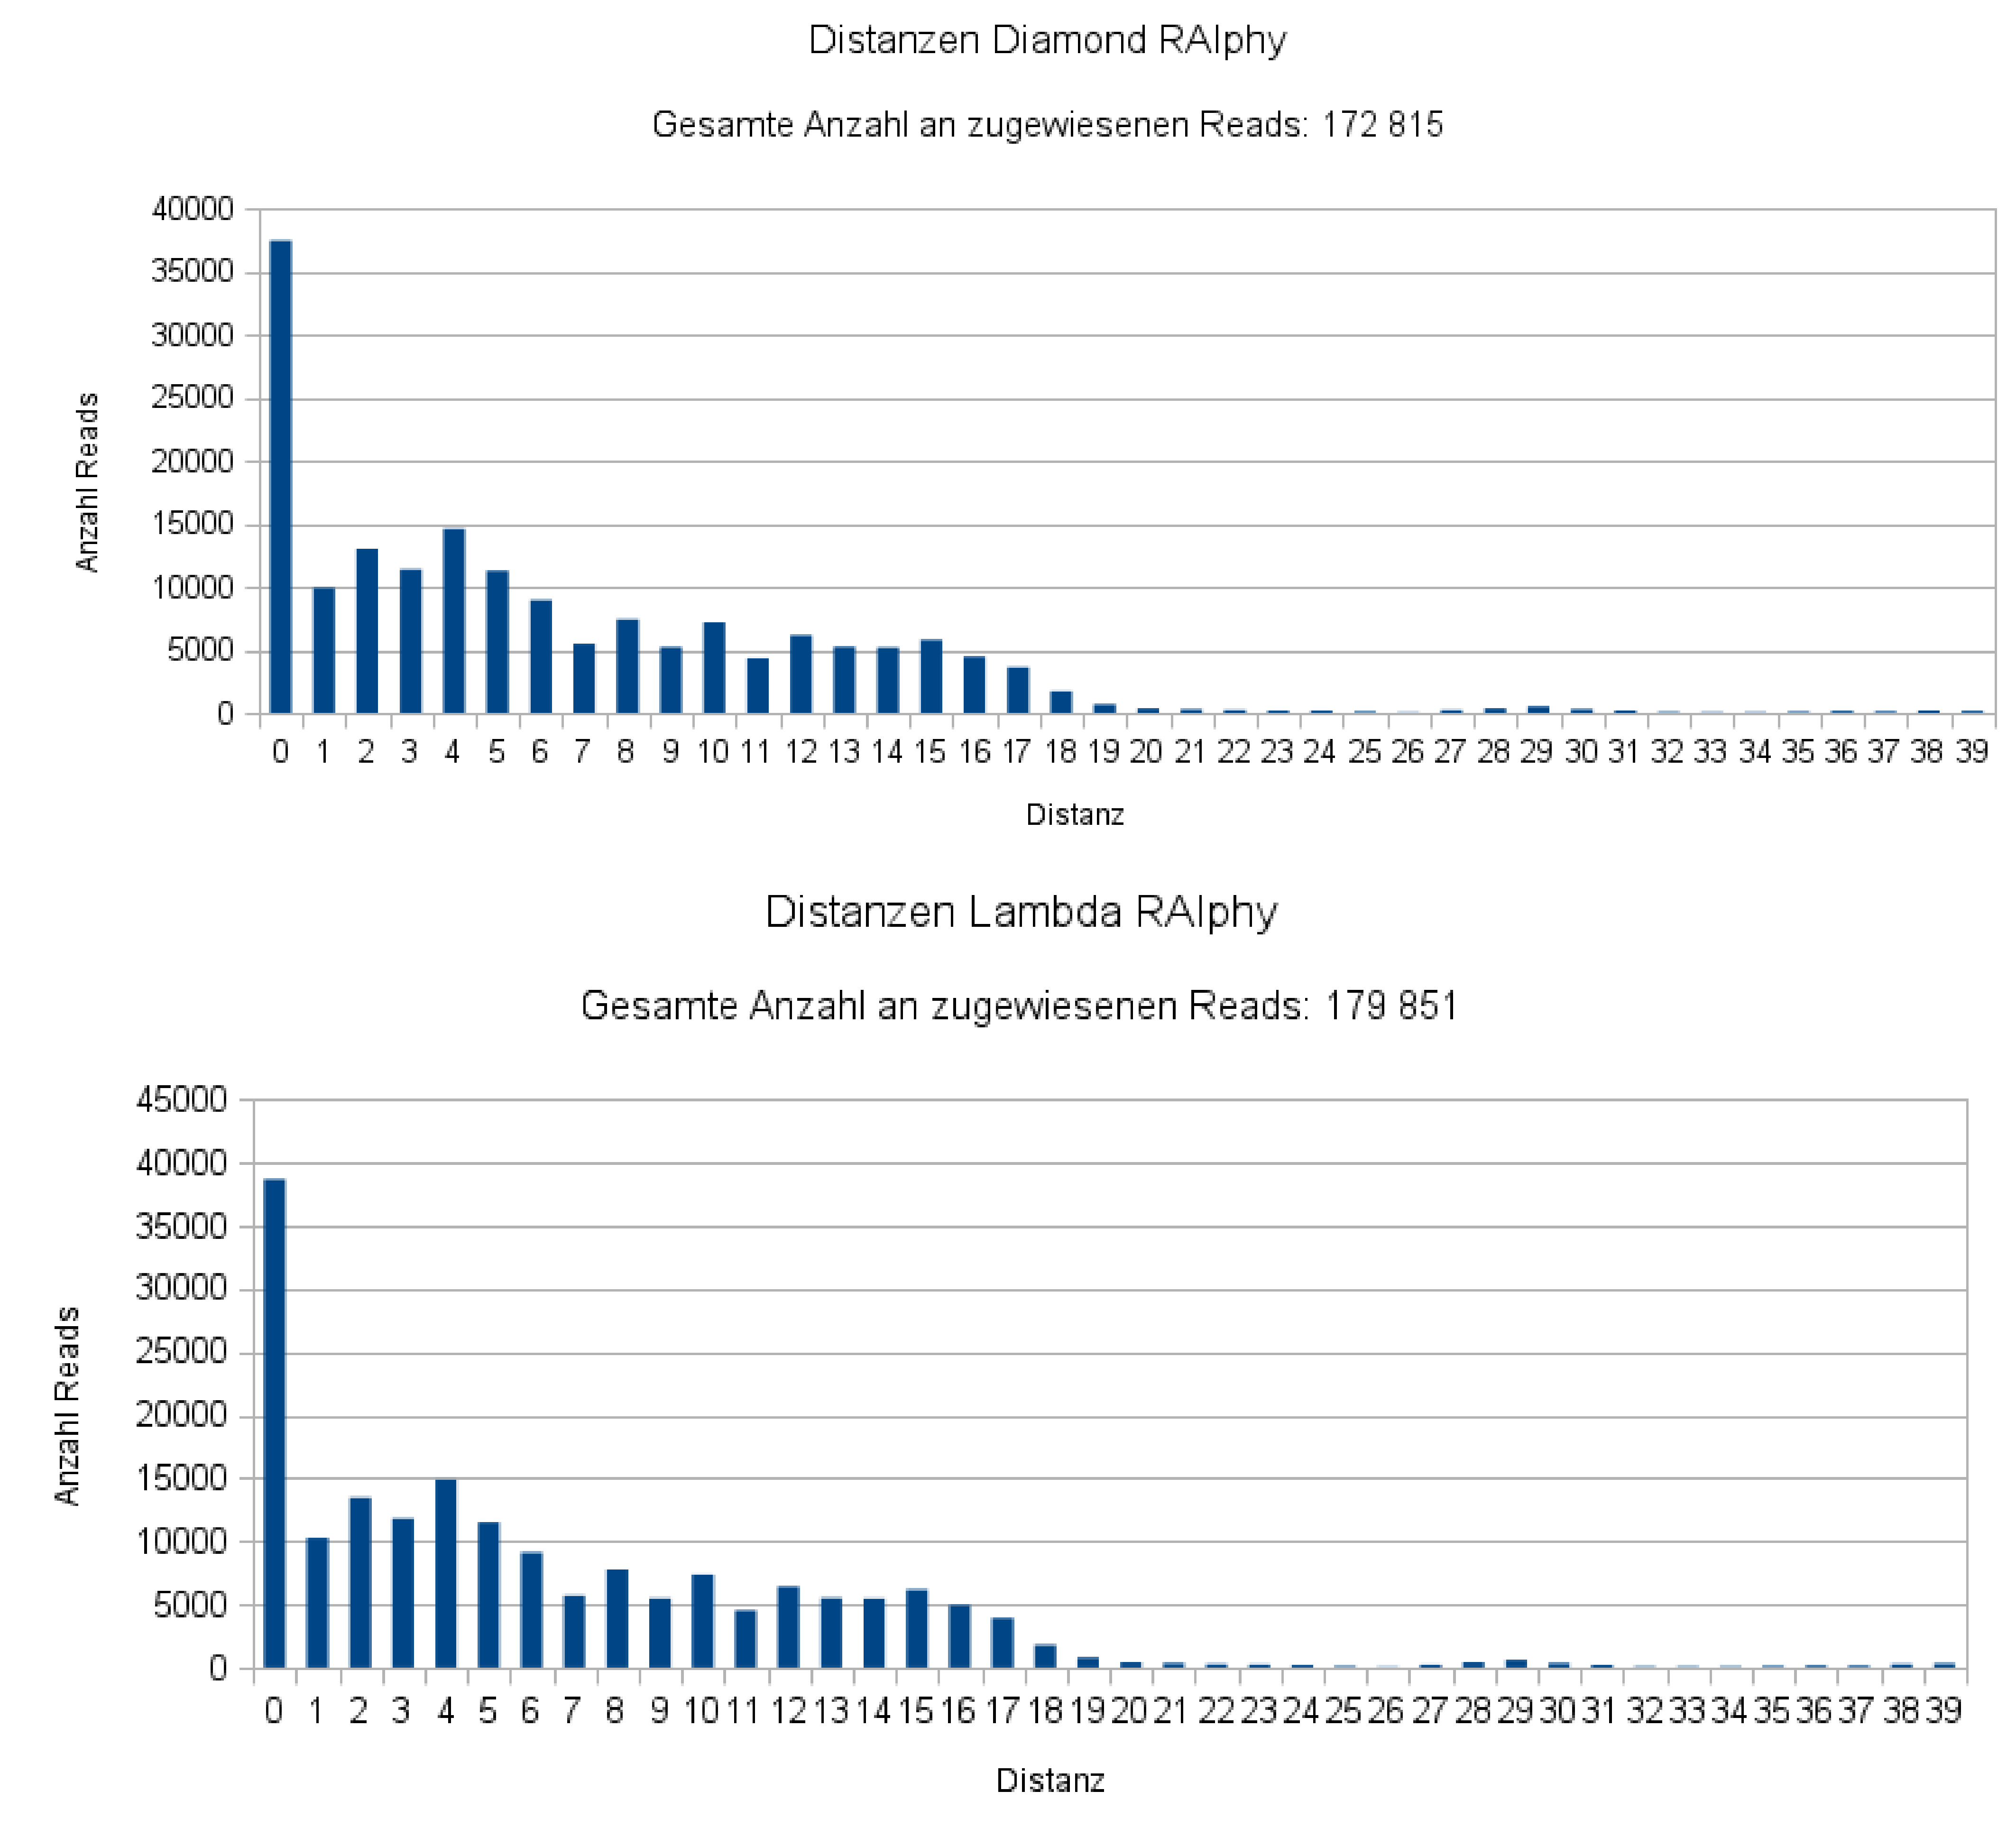
\includegraphics[width=\linewidth,height=15cm,
      keepaspectratio]{Abbildungen/RAIphy_Distanzen_both.png}
      \caption[Distanzverteilung der Reads: RAIphy Datensatz.]{\small{Distanzverteilung der Reads: RAIphy Datensatz.\newline \textbf{Oben}: Ausgabe Diamond. \textbf{Unten}: Ausgabe Lambda.}}
    \end{figure}
    
    F\"ur alle Datens\"atze l\"asst sich erkennen, dass Lambda insgesamt 
    mehr Reads zugeordnet hat als Diamond.
    \newpage
     \subsection{Sensitivit"at und Pr"azision}
       Die oben beschriebene Tendenz (Kapitel 3.1) zeigt sich auch f"ur die Genauigkeitsberechnungen. Die ausgewertete Lambda-Ausgabe zeigt f"ur den Datensatz FACS (Tab. 2) erst bei Distanzen ab 2 nennenswerte  Sensitivit"at- und Pr"azisionswerte, Carma (Tab. 1) und PhyloPythia (Tab. 3) sogar erst ab Distanzen von 4 - 5. Diamond dagegen weist bei den drei gennanten Datens"atzen schon bei einer Distanz von 0 auswertbare Genauigkeitsergebnisse auf.
     
     \begin{table}[H]
        \begin{tabular}{clllllll}
        &&&&&&\\
          \textbf{Distanz}&0&$\leq1$&$\leq2$&$\leq3$&$\leq4$&$\leq5$\\
          \textbf{Programm}&&&&&\\ \hline  
          &&&&&&\\
          Lambda&0&0&0&0&0,0128&0,0170\\
          Diamond&0,0386&0,0677&0,1047&0,1413&0,1688&0,1865\\
        \end{tabular}

        \begin{tabular}{clllllll}
          &&&&&&\\
          \textbf{Distanz}&0&$\leq1$&$\leq2$&$\leq3$&$\leq4$&$\leq5$\\
          \textbf{Programm}&&&&&\\ \hline  
          &&&&&&\\
          Lambda&0&0&0&0&0,0456&0,0606\\
          Diamond&0,1437&0,2521&0,3898&0,5262&0,6284&0,6944\\
        \end{tabular}
        \newline
        \caption[Genauigkeitsberechnung der Reads: Carma Datensatz.] {\small{Genauigkeitsberechnung der Reads: Carma Datensatz.\newline \textbf{Oben}: Sensitivit"at. \textbf{Unten}: Pr"azision.}} 
        
      \end{table}
         \begin{table}[H]
        \begin{tabular}{clllllll}
          &&&&&&\\
          \textbf{Distanz}&0&$\leq1$&$\leq2$&$\leq3$&$\leq4$&$\leq5$\\
          \textbf{Programm}&&&&&\\ \hline  
          &&&&&&\\
          Lambda&0&0&0,0016&0,0017&0,0021&0,0148\\
          Diamond&0,0736&0,0107&0,1358&0,1464&0,1696&0,1802\\
        \end{tabular}

        \begin{tabular}{clllllll}
        &&&&&&\\
          \textbf{Distanz}&0&$\leq1$&$\leq2$&$\leq3$&$\leq4$&$\leq5$\\
          \textbf{Programm}&&&&&\\ \hline  
          &&&&&&\\
          Lambda&0&0&0,0060&0,0063&0,0078&0,0550\\
          Diamond&0,2936&0,4280&0,5418&0,5842&0,6770&0,7194\\
        \end{tabular}
        \newline
        \caption[Genauigkeitsberechnung der Reads: FACS Datensatz.]{\small{Genauigkeitsberechnung der Reads: FACS Datensatz.\newline \textbf{Oben}: Sensitivit"at. \textbf{Unten}: Pr"azision.} }
         \end{table}

      \begin{table}[H]
        \begin{tabular}{clllllll}
          \textbf{Distanz}&0&$\leq1$&$\leq2$&$\leq3$&$\leq4$&$\leq5$\\
          \textbf{Programm}&&&&&\\ \hline
          &&&&&&\\ 
          Lambda&0&0&0&0&0&0,1101\\
          Diamond&0,0605&0,0847&0,1060&0,1182&0,1262&0,1388\\
        \end{tabular}

         \begin{tabular}{clllllll}
         &&&&&&\\
          \textbf{Distanz}&0&$\leq1$&$\leq2$&$\leq3$&$\leq4$&$\leq5$\\
          \textbf{Programm}&&&&&\\ \hline 
          &&&&&&\\
          Lambda&0&0&0&0&0&0,1892\\
          Diamond&0,1098&0,1538&0,1925&0,2146&0,2291&0,2519\\
        \end{tabular}
        \caption[Genauigkeitsberechnung der Reads: PhyloPythia Datensatz.]{\small{Genauigkeitsberechnung der Reads: PhyloPythia Datensatz.\newline \textbf{Oben}: Sensitivit"at. \textbf{Unten}: Pr"azision.} }
      \end{table}
     
     Die drei "ubrbigen Datens"atze Metaphyler (Tab. 4), PhymmBL (Tab. 5) und RAIphy (Tab. 6) zeigen sowohl bei der Sensitivit"at, als auch bei der Pr"azisionsberechnung f"ur Diamond und Lambda nahezu identische Ergebnisse.
      \begin{table}[H]
        \begin{tabular}{clllllll}
          \textbf{Distanz}&0&$\leq1$&$\leq2$&$\leq3$&$\leq4$&$\leq5$\\
          \textbf{Programm}&&&&&\\ \hline  
          &&&&&&\\
          Lambda&0,0004&0,0004&0,0004&0,0074&0,1380&0,1557\\
          Diamond&0,0004&0,0004&0,0004&0,0074&0,1378&0,1555\\
        \end{tabular}

        \begin{tabular}{clllllll}
        &&&&&&\\
          \textbf{Distanz}&0&$\leq1$&$\leq2$&$\leq3$&$\leq4$&$\leq5$\\
          \textbf{Programm}&&&&&\\ \hline  
          &&&&&&\\
          Lambda&0,00270&0,0270&0,0029&0,0459&0,8504&0,9594\\
          Diamond&0,00260&0,0026&0,0028&0,0462&0,8498&0,9588\\
        \end{tabular}
        \caption[Genauigkeitsberechnung der Reads: Metaphyler Datensatz.]{\small{Genauigkeitsberechnung der Reads: Metaphyler Datensatz.\newline \textbf{Oben}: Sensitivit"at. \textbf{Unten}: Pr"azision.} }
      \end{table}
    .
      \begin{table}[H]
        \begin{tabular}{clllllll}
          \textbf{Distanz}&0&$\leq1$&$\leq2$&$\leq3$&$\leq4$&$\leq5$\\
          \textbf{Programm}&&&&&\\ \hline  
          &&&&&&\\
          Lambda&0&0&0&0,0003&0,0026&0,0168\\
          Diamond&0&0&0&0,0003&0,0025&0,0159\\
        \end{tabular}

        \begin{tabular}{clllllll}
        &&&&&&\\
          \textbf{Distanz}&0&$\leq1$&$\leq2$&$\leq3$&$\leq4$&$\leq5$\\
          \textbf{Programm}&&&&&\\ \hline  
          &&&&&&\\
          Lambda&0&0&0&0,0011&0,0100&0,0637\\
          Diamond&0&0&0&0,0011&0,0100&0,0635\\
        \end{tabular}
        \caption[Genauigkeitsberechnung der Reads: PhymmBL Datensatz.]{\small{Genauigkeitsberechnung der Reads: PhymmBL Datensatz.\newline \textbf{Oben}: Sensitivit"at. \textbf{Unten}: Pr"azision.} }
      \end{table}

      \begin{table}[H]
        \begin{tabular}{clllllll}
          \textbf{Distanz}&0&$\leq1$&$\leq2$&$\leq3$&$\leq4$&$\leq5$\\
          \textbf{Programm}&&&&&\\ \hline  
          &&&&&&\\
          Lambda&0,0811&0,1026&0,1308&0,1555&0,1867&0,2108\\
          Diamond&0,0785&0,0993&0,1266&0,1504&0,1810&0,2046\\
        \end{tabular}

        \begin{tabular}{clllllll}
        &&&&&&\\
          \textbf{Distanz}&0&$\leq1$&$\leq2$&$\leq3$&$\leq4$&$\leq5$\\
          \textbf{Programm}&&&&&\\ \hline  
          &&&&&&\\
          Lambda&0,2151&0,2721&0,3470&0,4126&0,4954&0,5593\\
          Diamond&0,2167&0,2741&0,3494&0,4152&0,4996&0,5648\\
        \end{tabular}
        \caption[Genauigkeitsberechnung der Reads: RAIphy Datensatz.]{\small{Genauigkeitsberechnung der Reads: RAIphy Datensatz.\newline \textbf{Oben}: Sensitivit"at. \textbf{Unten}: Pr"azision.} }
      \end{table}
         
    \subsection{Laufzeitverhalten}
	Der direkte Vergleich der Laufzeiten von Lambda und Diamond l"asst 				erkennen, dass Diamond insgesamt bis zu drei Mal schneller l"auft als
	Lambda (Tab. 7). Lediglich f"ur die kleinen Datens"atze Carma und
	FACS ist Lambda schneller.\newline   
  
    \begin{table}[H]
        \begin{tabular}{lrrrr}
          \textbf{Datensatz}&Lambda [s]&Diamond [s]&Lambda [$\frac{s}{Mbp}$]&Diamond [$\frac{s}{Mbp}$]\\ \hline
          &&&&\\  
          Carma&\numprint{37}&\numprint{68}&\numprint{5}&\numprint{10}\\
          FACS&\numprint{39}&\numprint{72}&\numprint{5}&\numprint{10}\\
          PhyloPythia&\numprint{955}&\numprint{280}&\numprint{9}&\numprint{3}\\
          Metaphyler&\numprint{1255}&\numprint{788}&\numprint{31}&\numprint{19}\\
          PhymmBL&\numprint{362}&\numprint{176}&\numprint{19}&\numprint{9}\\
          RAIphy&\numprint{1512}&\numprint{538}&\numprint{14}&\numprint{5}\\  
        \end{tabular}   
        \caption{Laufzeitverhalten der Programme Diamond und Lambda f"ur die
        jeweiligen Datens"atze in Sekunden und Sekunden pro Megabase}
      \end{table}    
  \newpage 
  \section{Diskussion}
    Lambda und Diamond sind Programme, die eine Alternative zu dem 					Alignierprogramm BlastX \cite{altschul1990} darstellen sollen 					\cite{hauswedell2014, buchfink2014}. F"ur eine erste Quantifizierung 			dieser
    Aussage wurden im Rahmen dieses Projektes beide Programme miteinander
    verglichen. Angelehnt war der Vergleich auf der Arbeit von Bazinet 				und Cummings, 2012 \cite{bazinet2012}. Die Versuche wurden mit
    den gleichen Datensets durchgef"uhrt, die auch im "Vorlagepaper" 
    verwendet wurden. Es wird jedoch nicht angegeben, wie die Autoren 				vorgegangen sind um die Pr"azision, Sensitivit"at und das 						Laufzeitverhalten der von ihnen
    untersuchten Programme zu berechnen. Aus diesem Grund wurde in diesem 			Projekt eine eigene L"osung der Berechnung der Genauigkeit und des 
    Laufzeitverhaltens der Programme Lambda und Diamond erstellt. Die 				Ergebnisse lassen sich demnach nicht direkt mit den Ergebnissen von 			Bazinet und Cummings vergleichen. Es wurde entschieden, dass die 				Ergebnisse dieses Projektes unabh"angig vom "Vorlagepaper" betrachtet 			werden.
    \subsection{Distanzverteilung, Sensitivit"at und Pr"azision} 
      Die Ergebnisse bez"uglich der Distanzverteilung, Sensitivit"at und 
      Pr"azision zeigen, dass Diamond genauer ist als Lambda. Diamond 				  aligniert
      bei allen Datensets (bis auf PhymmBL und Metaphyler) den Gro{\ss}teil
      der untersuchten Reads mit den dem Gold-Standart entsprechenden 				  Sequenzen (Distanz von 0) und ist zudem f"ur die Datensets Carma, FACS 		  und PhyloPythia deutlich sensitiver und pr"aziser als Lambda.            
    
    \newpage
    \newpage
    
    \invisiblesection{Literaturverzeichnis}
    \begin{thebibliography}{14}
    
       \bibitem{altschul1990}
      Altschul, S.F., Gish, W., Miller, W., Myers, E.W. \& Lipman, D.J. (1990) 	  "Basic local alignment search tool." J. Mol. Biol. 215:403-410.
    
      \bibitem{bairoch2004}
	  Bairoch, A., Boeckmann, B., Ferro, S., Gasteiger, E. 2004, Swiss-Prot: 		  juggling between evolution and stability. Brief Bioinform. 539–55
	  
	  \bibitem{bazinet2012}
	  A. L. Bazinet and M. P. Cummings. \textit{A comparative evaluation of 		  sequence classification programs}. BMC Bioinformatics, 13: p92, 2012.
	  
	  \bibitem{bradysalzberg2009}
	  Brady A, Salzberg SL: Phymm and PhymmBL: metagenomic phylogenetic 			  classification with interpolated Markov models. Nat Methods 2009, 			  6(9):673-U68. 10.1038/nmeth.1358
	  
	  \bibitem{buchfink2014}
      Buchfink B., Xie C., Huson D.H.
	  Fast and sensitive protein alignment using DIAMOND. Nat. Methods 				  2014;12:59-60.
	  
	  \bibitem{dethlefsen2008} L. Dethlefsen, S. Huse, M. L. Sogin, and D. A. 	      Relman. The pervasive effects of an
	  antibiotic on the human gut microbiota, as revealed by deep 16S rRNA 			  sequencing. PLoS Biol., 6:e280, Nov 2008.
	  
	  \bibitem{GerlachStoye2011}
	  Gerlach W, Stoye J: Taxonomic classification of metagenomic shotgun 			  sequences with CARMA3. Nucleic Acids Res 2011, 39(14):e91. 					  10.1093/nar/gkr225
  
	  \bibitem{handelsman1998} 
      Jo Handelsman, Michelle R. Rondon, Sean F. Brady, Jon Clardy and Robert   	  M.Goodman. \textit{Molecular biological access to the chemistry of 			  unknown soil microbes: a new frontier for natural products}. Chemistry 		  \& Biology, 5(10): 245-249, 1998.
      
      \bibitem{hauswedell2014}
      Lambda: the local aligner for massive biological data; Hannes 				  Hauswedell, Jochen Singer, Knut Reinert; Bioinformatics 2014 30 (17): 		  i349-i355; doi: 10.1093/bioinformatics/btu439
      
      \bibitem{huson2011}
       Daniel H Huson, Suparna Mitra, Nico Weber, Hans-Joachim Ruscheweyh, and 	   Stephan C Schuster. Integrative analysis of environmental sequences 			   using MEGAN4. Genome Research, 21:1552–1560, 2011.
      
      
      \bibitem{Liu2010}
	  Liu B, Gibbons T, Ghodsi M, Pop M: MetaPhyler: Taxonomic profiling for 		  metagenomic sequences. In IEEE International Conference on 					  Bioinformatics and Biomedicine (BIBM). , Hong Kong; 2010:95–100.
	  
	  \bibitem{nalbantoglu2011}
	  Nalbantoglu OU, Way SF, Hinrichs SH, Sayood K: RAIphy: phylogenetic 			  classification of metagenomics samples using iterative refinement of 			  relative abundance index profiles. BMC Bioinf 2011, 12: 41. 					  10.1186/1471-2105-12-41
	  
	  \bibitem{patil2011}
	  Patil KR, Haider P, Pope PB, Turnbaugh PJ, Morrison M, Scheffer T, 			  McHardy AC: Taxonomic metagenome sequence assignment with structured 			  output models. Nat Methods 2011, 8(3):191–192. 10.1038/nmeth0311-191
		 
	  
	  \bibitem{stranneheim2010}
	  Stranneheim H, Kaller M, Allander T, Andersson B, Arvestad L, Lundeberg 		  J: Classification of DNA sequences using Bloom filters. Bioinformatics 		  2010, 26(13):1595–1600. 10.1093/bioinformatics/btq230
	  
	  	 
	  

    \end{thebibliography}


\end{document}




